\chapter{Revisão da Literatura}
\label{cap:revisao}

Com o intuito de estabelecer o estado da arte acerca dos métodos de percepção veicular baseados em sinais de sensores inerciais, foi conduzida uma Revisão Sistemática da Literatura (RSL) guiada pelos procedimentos descritos em \cite{kitchenham2009} e \cite{biolchini2005}. Esta revisão foi publicada em sua forma completa em \cite{menegazzo2018}, com a compilação de dados extraídos dos estudos selecionados e a descrição detalhada de cada trabalho em ordem cronológica de publicação. Baseado na revisão, foi publicado também em \cite{menegazzo2020} um Mapeamento Sistemático da Literatura (MSL) das abordagens e métodos no estado da arte. Nesta seção, é apresentada a sistemática aplicada na busca e seleção de estudos primários, assim como detalhado a análise produzida e as lacunas de pesquisa encontradas, as quais se pretende explorar nesta pesquisa. 

\section{Definições da Busca}

Na construção do protocolo que guiou a revisão sistemática, foram formuladas as seguintes \textbf{perguntas de pesquisa}:

\begin{enumerate}
\item Quais os métodos aplicados no processamento de sinais de sensores inerciais para gerar percepção veicular?
\item Quais são os padrões reconhecidos e suas classificações?
\item Quais as variáveis utilizadas e os fatores de dependência do modelo?
\item Quais sensores foram utilizados, suas características e configurações? Incluindo sensores não inerciais relacionados aos fatores de dependência.
\item Como os sensores foram distribuídos e posicionados no veículo?
\item Quais foram as aplicações finais das percepções veiculares desenvolvidas?
\end{enumerate}

Com estas questões propostas, buscou-se identificar o contexto no qual a amostragem de sinais ocorreu, os sensores utilizados, suas configurações e colocação no veículo. Estas informações são muito importantes para verificar a sensibilidade dos sensores, taxas de amostragem, referenciais e condições gerais de análise. Nos dados amostrados, foram analisadas as etapas de processamento realizadas e quais métodos foram aplicados para filtragem de sinais, reorientação de eixos e reconhecimento de padrões. Adicionalmente aos métodos, foram identificados os padrões de percepção veicular, as variáveis dos modelos e seus fatores de dependência, os quais afetam diretamente a adaptabilidade e portabilidade da solução. Desta forma, o seguinte escopo de revisão foi definido:

\begin{description}
\item[Objetivo:] Identificar e analisar métodos baseados em sensoriamento inercial para geração de percepção veicular.
\item[Controle:] Coleção de artigos relacionados ao objeto de pesquisa, obtidos por meio de revisão exploratória anterior.
\item[Intervenção:] Métodos e técnicas para reconhecimento e classificação de padrões em sinais unidimensionais.
\item[População:]Publicações relacionadas a projetos de sensoriamento veicular que usam acelerômetro ou giroscópio para reconhecer o ambiente em que o veículo está trafegando ou seu comportamento de condução.
\item[Resultados:] Lista de métodos e técnicas utilizadas no reconhecimento de padrões a partir de sinais inerciais para produzir percepção veicular.
\item[Aplicações:] Projetos de sensoriamento veicular em ITS, como agentes de navegação autônoma, ADAS, aplicativos de caixa preta, sistemas de \textit{mobile crowdsensing} e outros.
\end{description}

Após definir o objeto de pesquisa e o escopo da revisão, foram selecionadas as fontes nas quais os estudos primários foram buscados. A seleção das fontes seguiu os critérios de estar disponível na Internet, ser banco de dados científicos da área e possuir mecanismos avançados de busca baseados na composição lógica de palavras-chave e restrições de campos de documentos. Portanto, três fontes foram selecionadas, detalhadas na \autoref{tabela:definicao_pesquisa}. 

\begin{table}[h!]
    \small
    \centering
    \caption{Definições da busca}
    \label{tabela:definicao_pesquisa}
    \begin{tabular}{l}
        \toprule
        \textbf{Fontes} \\
        \toprule
        1. IEEE Xplore Digital Library \\
        2. ACM Digital Library \\
        3. Science Direct \\
        \toprule
        \textbf{Critérios de Inclusão}\\
        \toprule
        1. Artigos publicados e disponíveis integralmente em bases de dados científicas digitais.\\
        2. Trabalhos recentes publicados nos últimos sete anos (2013-2019).\\ 
        3. Artigos publicados no idioma inglês.\\
        4. Artigos que reconhecem algum padrão de percepção veicular em sinais de sensores inerciais.\\
        \toprule
        \textbf{Critérios de Exclusão}\\
        \toprule
        1. Artigos que não estão disponíveis integralmente nas fontes pesquisadas.\\
        2. Artigos que não foram publicados nos últimos sete anos (2013-2019).\\
        3. Artigos que não usam sensores inerciais para reconhecimento de padrões.\\
        4. Artigos que não usam sensores inerciais com três eixos.\\
        5. Artigos que não realizam reconhecimento da percepção veicular. \\
        6. Artigos de sensoriamento inercial para veículos de qualquer tração que não sejam mecânicos. \\
        7. Artigos que usam tecnologias intrusivas ou ativas.\\
        8. Artigos em outros idiomas, não incluídos no protocolo.\\
        \bottomrule
    \end{tabular}
    \fonte{Desenvolvido pelo autor.}
\end{table}

Para obter estudos primários a partir das bases de dados científicas definidas, com base nas palavras-chave obtidas nos estudos de controle foram construídas inicialmente as \textit{strings} de busca, detalhados nas Tabelas \ref{tabela:percepcao_ambiente_busca} e \ref{tabela:propriocepcao_busca}. Essas \textit{strings} foram modeladas de acordo com as características de cada fonte. Posteriormente, as \textit{strings} foram submetidas ao respectivo mecanismo de busca e seus resultados analisados por meio de uma estratégia de seleção. No processo de seleção, foram aceitos para a revisão os trabalhos que atenderam a todos os critérios de inclusão e a nenhum dos critérios de exclusão, detalhados na Tabela \ref{tabela:definicao_pesquisa}.

\begin{table}[h!]
    \caption{\textit{Strings} de busca para exterocepção veicular}
    \label{tabela:percepcao_ambiente_busca}
    \centering
    \small
    \begin{tabular}{l l}
        
        \toprule
        \textbf{Fonte} & IEEE Xplore Digital Library \\
        \midrule
        \textbf{\textit{String}} & ((Road \textbf{OR} Pavement \textbf{OR} Pothole \textbf{OR} Hole \textbf{OR} Bump \textbf{OR} "Speed Breaker") \\ \textbf{de Busca} &  \textbf{AND} (Accelerometer \textbf{OR} Gyroscope \textbf{OR} "Inertial Sensor")) \\
        \midrule
        \textbf{Filtros} & Intervalo: 2013-2019. Busca apenas em metadados. \\
        \bottomrule
        
        \\
        
        \toprule
        \textbf{Fonte} & ACM Digital Library \\
        \midrule
        \textbf{\textit{String}} & ((Road \textbf{OR} Pavement \textbf{OR} Pothole \textbf{OR} Bump \textbf{OR} Speed Breaker") \textbf{AND} \\ \textbf{de Busca} & " (Accelerometer \textbf{OR} Gyroscope \textbf{OR} "Inertial Sensor")) \\ 
        \midrule
        \textbf{Filtros} & Intervalo: 2013-2019. Busca em títulos e resumos. \\ 
        \bottomrule
        
        \\
        
        \toprule
        \textbf{Fonte} & Science Direct \\
        \midrule
        \textbf{\textit{String}} & ((Road \textbf{OR} Pavement \textbf{OR} Pothole \textbf{OR} Hole \textbf{OR} Bump \textbf{OR} "Speed Breaker") \\ \textbf{de Busca} &  \textbf{AND} (Accelerometer \textbf{OR} Gyroscope \textbf{OR} "Inertial Sensor")) \\ 
        \midrule
        \textbf{Filtros} & Intervalo: 2013-2019. Busca em títulos, resumos e palavras-chave. \\
        \bottomrule
    \end{tabular}
    \fonte{Desenvolvido pelo autor.}
\end{table}

\begin{table}[h!]
    \caption{\textit{Strings} de busca para propriocepção veicular}
    \label{tabela:propriocepcao_busca}
    \centering
    \small
    \begin{tabular}{l l}
        
        \toprule
        \textbf{Fonte} & IEEE Xplore Digital Library \\
        \toprule
        \textbf{\textit{String}} & (Driving Events \textbf{OR} Driving Patterns \textbf{OR} Driving Style \textbf{OR} Drive Behaviour) \textbf{AND} \\ \textbf{de Busca} & (Accelerometer \textbf{OR} Gyroscope \textbf{OR} “Inertial Sensor”) \\
        \toprule
        \textbf{Filtros} & Intervalo: 2013-2019. Busca apenas em metadados. \\
        \bottomrule
        
        \\
        
        \toprule
        \textbf{Fonte} & ACM Digital Library \\
        \toprule
        \textbf{\textit{String}} & ("Driving Events" \textbf{OR} "Driving Patterns" \textbf{OR} "Driving Style" \textbf{OR} "Drive Behaviour")  \textbf{AND}  \\ \textbf{de Busca} & (Accelerometer \textbf{OR} Gyroscope \textbf{OR} "Inertial Sensor") \\
        \toprule
        \textbf{Filtros} & Intervalo: 2013-2019.  Busca em títulos e resumos. \\
        \bottomrule
         
         \\
         
        \toprule
        \textbf{Fonte} & Science Direct \\
        \toprule
        \textbf{\textit{String}} & (Driving Events \textbf{OR} Driving Patterns \textbf{OR} Driving Style \textbf{OR}  Drive Behaviour) \textbf{AND} \\ \textbf{de Busca} & (Accelerometer \textbf{OR} Gyroscope \textbf{OR} “Inertial Sensor”) \\
        \toprule
        \textbf{Filtros} & Intervalo: 2013-2019. Busca em títulos, resumos e palavras-chave. \\
        \bottomrule
        
    \end{tabular}
    \fonte{Desenvolvido pelo autor.}
\end{table}

\section{Execução da Busca}

Com as definições estabelecidas, foram realizadas buscas por estudos primários nas três fontes selecionadas. Devido à limitação de número de termos nos mecanismos de busca, foram realizadas duas buscas, uma para exterocepção e outra para propriocepção, conforme as \textit{strings} de busca construídas. A busca por exterocepção resultou em 737 artigos e a propriocepção em 239 artigos. Após análise dos estudos de acordo com os critérios estabelecidos, 66 artigos sobre exterocepção e 25 sobre propriocepção foram selecionados para esta revisão, conforme detalhado na Tabela \ref{tabela:resultados_sumarizados_busca}. 

\begin{table}[h]
    \caption{Resultados sumarizados das buscas}
    \label{tabela:resultados_sumarizados_busca}
    \centering
    \small
    \begin{tabular}{lcccc}
    \cmidrule(l){2-5} & \multicolumn{2}{c}{\textbf{Exterocepção}} & \multicolumn{2}{c}{\textbf{Propriocepção}} \\ \midrule
    \textbf{Fonte} & Recuperado & Selecionado & Recuperado & Selecionado \\ \midrule
    IEEE Xplore Digital Library & 619 & 51 & 196 & 21 \\ \midrule
    ACM Digital Library & 32 & 6 & 6 & 1 \\ \midrule
    Science Direct & 86 & 9 & 37 & 3 \\ \midrule
    \textbf{Total} & 737 & 66 & 239 & 25 \\ \bottomrule
    \end{tabular}
    \fonte{Desenvolvido pelo autor.}
\end{table}

\section{Análise do Estado da Arte}

Nesta seção é apresentada uma análise multi-aspecto e um mapeamento dos estudos analisados, principalmente em relação à abordagem, métodos e técnicas empregadas. Consideramos para esta revisão as etapas de coleta de dados, pré-processamento e processamento. Entretanto, existe também a etapa de pós-processamento, geralmente empregada com foco na aplicação final dos dados e métodos para melhorar a confiabilidade das percepções. Sendo assim, esta etapa não se mostra essencial nesta revisão, já que buscamos a confiabilidade nas três primeiras etapas, através de uma modelagem dos fatores de dependência. 

Nas próximas subseções são detalhadas cada uma das etapas analisadas. Inicialmente são explicados os referenciais para amostragem e análise de dados, juntamente com as técnicas de reorientação de eixos, que envolvem as etapas de coleta e pré-processamento dos dados. A seguir, são apresentados os fatores de dependência que interferem nos sinais amostrados, relacionados às propriedades sensoriais, veiculares, de condução e ambientais. Após, detalhamos as três etapas de análise. Na etapa de coleta de dados, são especificadas as plataformas de \textit{hardware} utilizadas, a colocação dos sensores e as configurações para amostragem do sinal. Na etapa de pré-processamento, são apresentados os métodos aplicados para remoção de ruído, suavização de sinal, extração de características e segmentação de dados. Na etapa de processamento, são discutidas as técnicas utilizadas para reconhecer as exterocepções e as propriocepções. Em seguida, são detalhados os padrões de percepção e suas classificações possíveis de serem gerados através de sensores inerciais, assim como suas aplicações finais. Na sequência, é apresentada a discussão e considerações acerca do estado da arte. Por fim, é discorrida uma análise comparativa detalhada do estado da arte das percepções específicas trabalhadas nesta pesquisa.

\subsection{Referenciais}

Os sensores inerciais não requerem nenhum referencial externo. Sendo assim, possuem seu próprio referencial, onde o sistema de coordenadas no qual os dados são amostrados é definido em relação a si próprios. No entanto, a análise dos dados com o objetivo de produzir percepção veicular deve ser realizada no referencial do veículo, como mostra a \autoref{fig:quadros_referencia}. Para isso, é necessário reorientar os eixos, mapeando os dados brutos de um sistema para outro.

\begin{figure}[h]
  \centering
  \caption{Referenciais: (a) Referencial do sensor. (b) Referencial do sensor interno a dispositivos móveis. (c) Referencial da Terra. (d) Referencial do veículo.}
   \label{fig:quadros_referencia}
   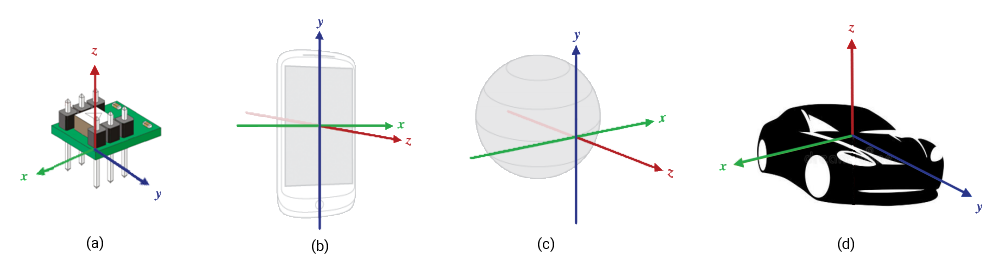
\includegraphics[width=1\textwidth]{figuras/fig_3.png}
   \fonte{Desenvolvido pelo autor.}
\end{figure}

A orientação dos dados é importante no processo de análise para que se possa utilizar os valores de acordo com o tipo de percepção a ser realizada. Sendo assim, baseando-se no referencial do veículo, os padrões de percepção de ambiente são geralmente mais evidentes na aceleração do eixo Z e na taxa de rotação dos eixos X e Y. Já quanto aos padrões de propriocepção, mostram-se mais evidentes nos dados de aceleração nos eixos X e Y e na taxa de rotação do eixo Z. Para uma padronização de nomenclatura neste trabalho, serão usados os termos definidos nas Tabelas \ref{table:accelerometer_reference_frames} e \ref{table:gyroscope_reference_frames} para se referir aos dados em relação a cada um dos referenciais.

\begin{table}[h]
    \caption{Referenciais para os dados de aceleração}
    \label{table:accelerometer_reference_frames}
    \centering
    \small
    \begin{tabular}{clll}
        \toprule
        \textbf{Axis} & \textbf{Sensor} & \textbf{Veículo} & \textbf{Mundo} \\
        \toprule
        X & Aceleração em X & Aceleração Lateral & Aceleração Leste \\
        \midrule
        Y & Aceleração em Y & Aceleração Longitudinal & Aceleração Norte \\
        \midrule
        Z & Aceleração em Z & Aceleração Vertical & Aceleração Vertical (Mundo) \\
        \bottomrule
    \end{tabular}
    \fonte{Desenvolvido pelo autor.}
\end{table}

\begin{table}[h]
    \caption{Referenciais para os dados de taxa de rotação}
    \label{table:gyroscope_reference_frames}
    \centering
    \small
    \begin{tabular}{clll}
        \toprule
        \textbf{Axis} & \textbf{Sensor} & \textbf{Veículo} & \textbf{Mundo} \\
        \toprule
        X & Taxa de Rotação Pitch & Taxa de Rotação Lateral & N/A \\
        \midrule
        Y & Taxa de Rotação Roll & Taxa de Rotação Longitudinal & N/A \\
        \midrule
        Z & Taxa de Rotação Yaw & Taxa de Rotação Vertical & N/A \\
        \bottomrule
    \end{tabular}
    \fonte{Desenvolvido pelo autor.}
\end{table}

Para a reorientação dos eixos, duas estratégias foram identificadas nos estudos revisados: o posicionamento controlado e o mapeamento através de fórmulas baseadas nos ângulos de Euler. O posicionamento controlado consiste em uma técnica simples, onde sensor é colocado no veículo de forma que os eixos nos referenciais coincidam, ou seja, os eixos do sensor ficam alinhados com os eixos do veículo. Portanto, não é necessário aplicar pré-processamento para reorientação. Essa técnica é usada tanto para os dados do acelerômetro e do giroscópio. 

Os ângulos de Euler, por sua vez, aplicados apenas aos dados de aceleração, fornecem um meio de representar a orientação espacial tridimensional de qualquer referencial como uma composição de três rotações elementares. A orientação de referência pode ser tomada como uma orientação inicial a partir da qual o sistema de coordenadas gira para alcançar sua orientação real \cite{Singh2017}. Assim, essas fórmulas reorientam os dados brutos usando os ângulos fornecidos. Estes dois métodos são detalhados e analisados comparados nas subseções de coleta de dados e pré-processamento. 

\subsection{Fatores de Dependência}

Os valores amostrados através dos sensores inerciais, embora não dependam de um referencial externo para sua produção, são afetados por propriedades externas e internas aos sensores. Essas propriedades constituem fatores de dependência, que influenciam diretamente a corretude, amplitude e dispersão dos valores medidos. Através da tanto da análise da literatura, quando de experimentos exploratórios conduzidos, foi possível observar a existência de fatores de dependência, classificados na forma de quatro propriedades relacionadas às variações contextuais discutidas abaixo. Para que uma solução desenvolvida possa ser adaptativa na forma que está sendo proposta, é necessário que o modelo considere todas estas propriedades no seu desenvolvimento.

\begin{description}
	
	\item [Propriedades Sensoriais:] 
	
	Quatro fatores de dependência estão relacionados às configurações e características dos sensores, sendo eles a orientação \cite{Kumar2017,Alam2020}, resolução, faixa de medição e taxa de amostragem. A orientação do sensor, conforme discutido na seção anterior, afeta a amostragem de dados no sistema de coordenadas correto. Portanto, o sensor deve ser colocado de forma a ficar alinhado com o sistema de coordenadas do veículo ou ter uma reorientação de eixos para esse referencial. Isso implica na confiabilidade dos dados existentes em cada eixo de análise, pois cada um deles visa atingir certa percepção veicular.

	O segundo e o terceiro fator estão fortemente correlacionados. A resolução é definida de acordo com a faixa de medição FSR escolhida para o sensor. Portanto, é necessário que o sensor tenha uma faixa de medição adequada para poder amostrar os dados sem saturar, ou seja, que a faixa de medição do sensor não seja menor que os valores possíveis a serem monitorados. A resolução, estabelecida a partir da faixa de valores a serem analisados, fornece o quão próximo o valor medido é comparado ao valor real, no processo de quantização e representação no sistema binário. Assim, devido à limitação do número de bits representado pelos sensores, quanto maior a faixa de medição, menor a resolução.
	
	Por fim, a taxa de amostragem descreve a frequência da coleta de dados por segundo. A escolha desse valor deve levar em consideração não apenas o custo computacional de armazenamento e processamento dos dados amostrados, mas também se, a uma determinada velocidade, será possível obter amostras suficientes para realizar as percepções. Dessa forma, quando o veículo está em alta velocidade, percepções transientes, como buracos, precisam de uma taxa de amostragem satisfatória, para que seja possível adquirir amostras suficientes desse evento.
	
	\item [Propriedades Veiculares:] 
	
	Relacionam-se a estrutura veicular. O principal fator de dependência é o sistema de suspensão \cite{Kumar2017, Wickramarathne2018,Alam2020}. Estes sistema, com o objetivo de amortecer os impactos causados pelas irregularidades e obstáculos na superfície da pista, faz com que os valores medidos sejam reduzidos dependendo da localização dos sensores na infraestrutura veicular. Desta forma, os valores medidos abaixo da suspensão apresentam interferência da massa não suspensa através da rigidez e absorção do pneu, e os medidos acima da suspensão adicionam também a influência da massa suspensa, através da mola e amortecedor \cite{Yafeai2019}. Desta forma, para poder realizar as percepções em diferentes veículos é necessário considerar que cada um deles possuí uma estrutura diferente, com diferentes sistemas de suspensão, e que diferentes colocações do sensor em um mesmo veículo pode ter mais ou menos interferência destas propriedades.

	\item [Propriedades de Condução:] 
	
	As propriedades de condução, intrinsecamente vinculadas as propriedades veiculares, relacionam-se aos diferentes estilos de condução do veículo.  Cada motorista possuí seu estilo de condução, aplicando mais ou menos aceleração, dirigindo velocidades mais altas ou mais baixas, realizando diferentes manobras \cite{Alam2020}. Cada um destes fatores impacta nos sinais amostrados, de acordo com a tração e direção aplicada e o modo com que o veículo interage com o ambiente. O principal fator de dependência é a velocidade longitudinal \cite{Brunauer2016,Douangphachanh2013,Gueta2017,Kumar2017,Lima2016,M.2017,Nalavde2015,Singh2017,Alam2020}, a qual possui duas principais implicações. Uma vez que as curvas são feitas em todos os eixos do sistema de coordenadas do veículo, ocorre a produção do componente de força centrífuga. Portanto, as acelerações medidas dependem diretamente da velocidade aplicada. A segunda implicação da velocidade está na distribuição no tempo dos valores amostrados. Em velocidades mais baixas, mais amostras do evento são coletadas e, com o veículo em velocidades diferentes, diferentes quantidades de amostras são obtidas.

	\item [Propriedades Ambientais:] 
	
	Estas propriedades relacionam-se com as características do ambiente externo ao veículo \cite{Alam2020}, as quais afetam diretamente os valores amostrados, de forma que uma mesma percepção possa ter padrões muito diferentes. Na classificação de tipo de superfície de pista, um determinado tipo de pavimento pode apresentar variações no estado de conservação, possuir buracos, lombadas, outras anomalias e obstáculos. A variação destas características não devem influenciar a classificação final. Na detecção de lombadas este tipo de obstáculo pode estar presente em pistas com diferentes pavimentações, como asfalto e paralelepípedo \cite{Masino2017}. Cada um destes tipos de pavimento apresentam diferentes padrões nos sinais nos sensores. Além disso, as lombadas podem apresentar variações em suas dimensões, seja pela forma como foram construídas ou pela falta de manutenção. Independente destas condições, estas variações não devem influenciar a classificação final, onde lombadas diferentes devem ser reconhecidas da mesma maneira.
	 
\end{description}

\subsection{Coleta de Dados}

A coleta de dados nos estudos analisados foi realizada em diferentes contextos, de acordo com o tipo de percepção que se pretendia produzir. Esses contextos envolviam estradas com diferentes pavimentos, estados de conservação, condições climáticas, irregularidades, obstáculos e modos de condução. De acordo com \autoref{fig:sensores_ocorrencia}, observamos que a maioria dos estudos utilizou apenas os dados do sensor acelerômetro, uma vez que este é mais facilmente encontrado em dispositivos móveis do que o giroscópio. No entanto, outras soluções foram propostas utilizando dados do giroscópio ou de ambos, embora em quantidade consideravelmente menor.

\begin{figure}[h!]
  \centering
  \caption{Sensores inerciais utilizados nos estudos revisados}
   \label{fig:sensores_ocorrencia}
   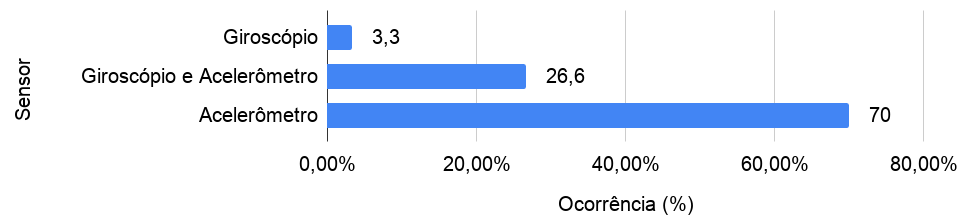
\includegraphics[width=0.85\textwidth]{figuras/fig_14.png}
   \fonte{Desenvolvido pelo autor.}
\end{figure}

Os estudos também foram agrupados de acordo com a plataforma utilizada, detalhada na \autoref{fig:plataformas_ocorrencia}. Aproximadamente 83\% dos estudos utilizou sensores inerciais embarcados em dispositivos móveis como \textit{smartphones} e \textit{tablets}, enquanto que apenas 17\% utilizaram anexado aos veículos. No uso de sensores em dispositivos móveis, as soluções propostas são mais vulneráveis a erros, pois os dispositivos não permanecem fixos o tempo todo, dependem de uma reorientação dos eixos e, geralmente, possuem sensores menos robustos. Em geral, essa abordagem tem sido utilizada em sistemas de \textit{mobile crowdsensing}, onde os dados produzidos localmente são enviados para um servidor remoto, que recebe percepções veiculares de várias fontes. Após o pós-processamento para melhorar a confiabilidade dos dados, as percepções retornam aos usuários em aplicativos de assistência ao motorista. Por sua vez, o uso de sensores anexados à veículos foi combinado com a utilização de SBC Raspberry Pi, ou microcontrolador, como o Arduíno, visando principalmente resultados locais com maior precisão e acurácia, sem a necessidade de processamento remoto ou dados de outras fontes.

\begin{figure}[h!]
  \centering
  \caption{Plataformas utilizadas nos estudos revisados}
   \label{fig:plataformas_ocorrencia}
   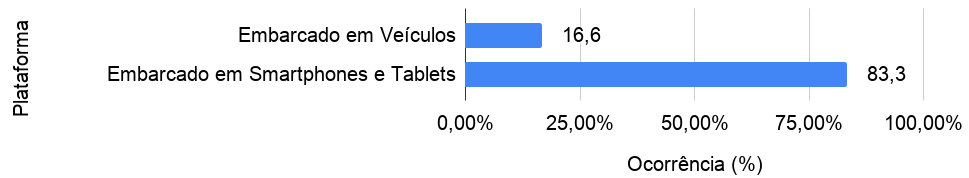
\includegraphics[width=0.85\textwidth]{figuras/fig_15.png}
   \fonte{Desenvolvido pelo autor.}
\end{figure}

Os sensores foram colocados no veículo de acordo com a plataforma utilizada. Sensores inerciais em dispositivos móveis foram colocados dentro da cabine, geralmente no painel de controle, bancos, próximo ao câmbio de marchas ou fixado com suporte no pára-brisas. Sensores embarcados no veículo foram colocados no painel, no chassi, nas rodas, próximo e abaixo da suspensão e próximo e acima da suspensão. A \autoref{fig:colocacao_sensores_ocorrencia} detalha os colocações encontradas. Devido à economia de recursos, especialmente a bateria, os dados dos sensores de dispositivos móveis foram coletados a uma taxa de amostragem na faixa de $Hz$, enquanto que os fixados no veículo utilizaram uma amostragem maior, na faixa de $KHz$. Além dos sensores inerciais, os estudos também utilizaram fontes de dados auxiliares, como magnetômetros, GPS e \textit{On-Board Diagnostic II} (OBD-II).

\begin{figure}[h!]
  \centering
  \caption{Colocação dos sensores no veículo}
   \label{fig:colocacao_sensores_ocorrencia}
   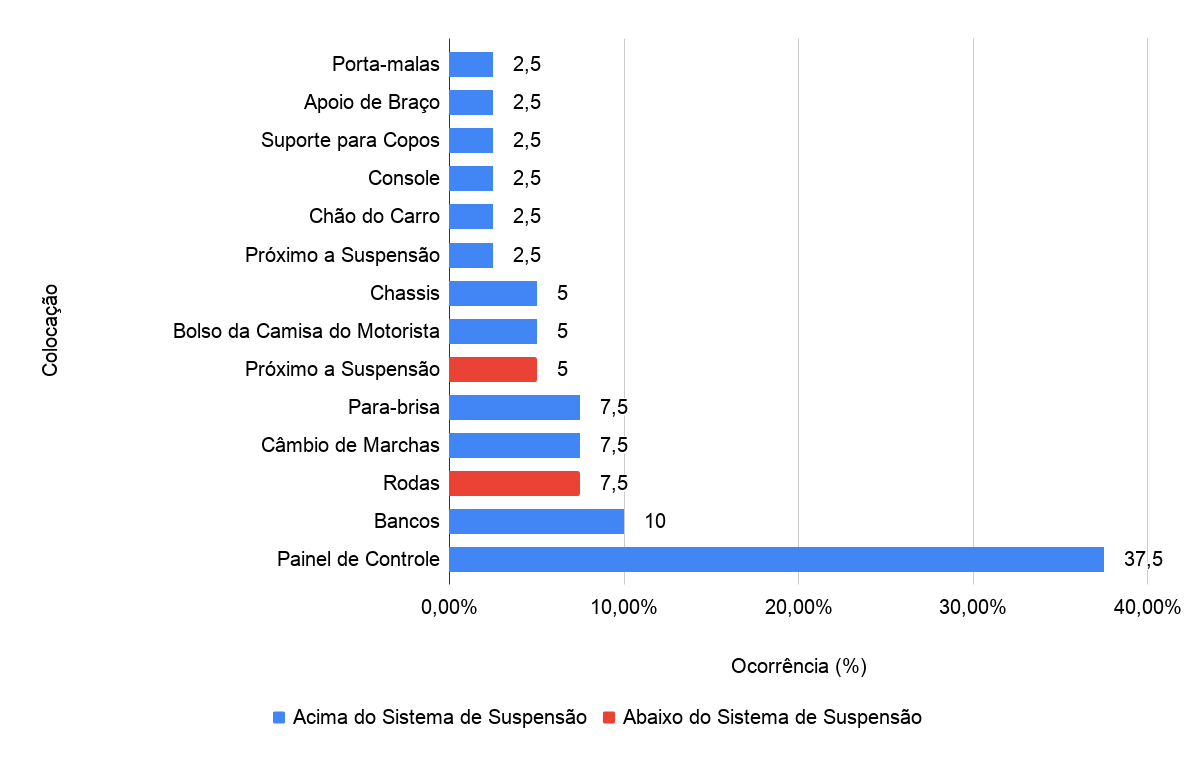
\includegraphics[width=1\textwidth]{figuras/fig_16.png}
   \fonte{Desenvolvido pelo autor.}
\end{figure}

\subsection{Pré-Processamento}

Após a coleta, os dados brutos foram pré-processados para serem parametrizados a técnica que reconhece e classifica os padrões de percepção. O pré-processamento foi subdividido em três fases, de acordo com sua finalidade. Na primeira, foram aplicados métodos para a reorientação de eixos. Na segunda, os dados foram ajustados para remoção de ruído, suavização de sinal, segmentação de dados e extração de características. Finalmente, na terceira fase, foram aplicados métodos para georreferenciamento dos dados.

Na primeira etapa de pré-processamento, poucos estudos utilizaram a reorientação dos eixos entre os sistemas de coordenadas, mapeando os dados entre os referenciais de coleta e análise. A maioria utilizou os dados no referencial amostrado, com os sensores posicionados de forma arbitrária. Dentre os que utilizaram reorientação de eixos, a maioria empregou fórmulas baseadas nos ângulos de Euler \cite{Li2018,Orhan2013,Singh2017,Vittorio2014,Vlahogianni2017}. Nesta técnica, os ângulos foram calculados de diferentes maneiras. Em \cite{Singh2017,Orhan2013,Vittorio2014} o referencial inicial foi estabelecido como estado estacionário ($x=0m/s^2$, $y=0m/s^2$ e $z=9.81m/s^2$), a partir do qual os ângulos de mapeamento foram calculados. Em \cite{Li2018} foi utilizado como estado inicial os valores do acelerômetro, medindo os ângulos continuamente. Em \cite{Singh2018} foi usado como estado inicial as médias individuais dos valores de aceleração nos três eixos, dos últimos 15 segundos, quando a magnitude total estava próxima a $9.8 \pm 0.2 m/s^2$. Todos eles empregaram como orientação final os valores atuais de aceleração.

Nos estudos analisados, os ângulos de Euler foram calculados com base na localização da gravidade, reorientando o eixo Z perpendicular ao plano do solo, apontando em direção ao céu. Para adicionar uma orientação aos dados dos eixos X e Y, alguns estudos utilizaram do sensor magnetômetro, que mede o campo geomagnético ambiental \cite{Sattar2018}. Desta forma, o eixo X se torna tangencial ao solo e aponta para o leste, enquanto o eixo Y também tangencial ao solo aponta para o polo norte geomagnético \cite{Sattar2018}. Alguns estudos anteriores também utilizaram o sensor de gravidade para cálculo da orientação inicial e final. Este sensor baseado em \textit{software} deriva seus dados através da fusão de dados do acelerômetro e do giroscópio, medindo a força gravitacional distribuída em cada um dos eixos físicos. Em suma, a utilização das fórmulas baseadas em ângulos de Euler mapeou os dados do acelerômetro para o referencial da terra, o qual sobrepõe apenas o eixo Z do referencial do veículo, e somente em situações de quando o veículo está em terreno plano.

Na segunda etapa de pré-processamento, várias técnicas foram aplicadas para ajustes nos sinais, mostradas na \autoref{fig:preprocessamento_sinais_ocorrencia}, utilizadas principalmente no domínio do tempo, embora outros domínios como frequência e tempo-frequência também tenham sido explorados, conforme detalha a \autoref{fig:dominios_analise_ocorrencia}. Abordagens estatísticas como Gaussiana \cite{Pooja2017}, \textit{Skewness} \cite{Alqudah2016}, \textit{Kurtosis} \cite{Alqudah2016}, Mediana \cite{Alqudah2016,Li2016}, \textit{Root Mean Square} (RMS) \cite{Jang2015,Li2018,Sharma2015}, Média/Média Móvel \cite{Alqudah2016,Andria2016,Bose2018,Li2016, Pholprasit2015,Savera2016,Singh2017}, Variância/Variância Móvel \cite{Alqudah2016,Andria2016} e Desvio Padrão \cite{Andria2016,BelloSalau2018,Hou2017,Lima2016,Pholprasit2015,Prapulla2017} foram utilizados no domínio do tempo para suavizar os sinais e extrair características dos dados de vibração. Entre as pesquisas que utilizaram pré-processamento de sinal, cerca de 60\% deles utilizaram métodos estatísticos. No domínio da frequência, os filtros \textit{Infinite Impulse Response} (IIR) \cite{Wu2018} e \textit{Butterworth} \cite{Hou2017,Niskanen2015,Pitonak2016,Souza2018,Wu2013} foram utilizados na remoção de componentes dos sinais. Já a \textit{Fast Fourier Transform} (FFT) \cite{Allouch2017,Douangphachanh2013,Douangphachanh2014} e \textit{Wavelets} \cite{BelloSalau2018,Eftekhari2018,El-Wakeel2018,Gueta2017,Singh2017,Wang2018} foram utilizadas na remoção de ruídos e extração de características. A segmentação dos dados foi realizada em janelas deslizantes em função do tempo \cite{Wang2018}, número de amostras \cite{Singh2017} ou distância \cite{Li2018}. 

\begin{figure}[h!]
  \centering
  \caption{Métodos utilizados no pré-processamento de sinais dos estudos revisados}
   \label{fig:preprocessamento_sinais_ocorrencia}
   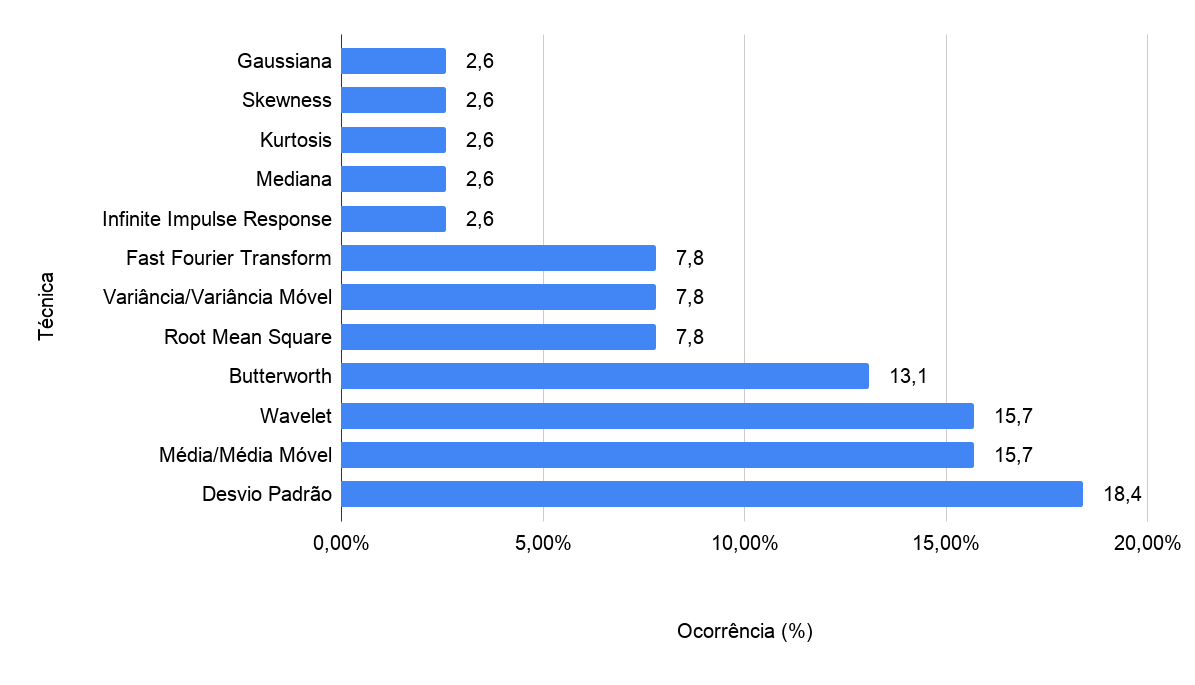
\includegraphics[width=1\textwidth]{figuras/fig_17.png}
   \fonte{Desenvolvido pelo autor.}
\end{figure}

\begin{figure}[h!]
  \centering
  \caption{Domínios de análise utilizados nos estudos revisados}
   \label{fig:dominios_analise_ocorrencia}
   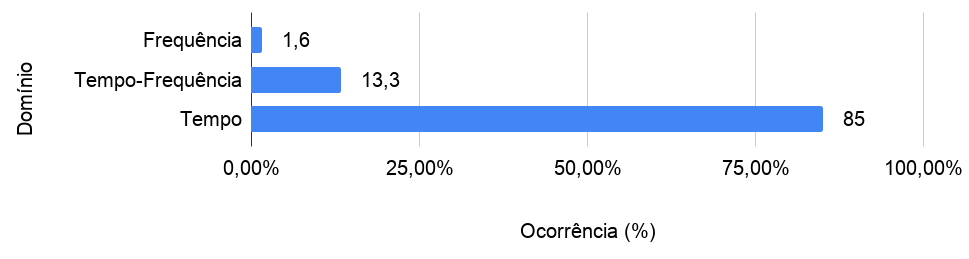
\includegraphics[width=0.85\textwidth]{figuras/fig_18.png}
   \fonte{Desenvolvido pelo autor.}
\end{figure}

Na última fase de pré-processamento, uma vez que a taxa de amostragem de dados dos sensores inerciais é muito mais rápida que a amostragem de dados de localização (1Hz), são necessárias técnicas para estimar a localização e velocidade antes da próxima amostra do GPS. Para isso, apenas \cite{Li2018} utilizou um tratamento, aplicando interpolação linear com os dados de aceleração para obter dados de localização com uma frequência maior. 

\subsection{Processamento}

Para reconhecer e classificar os padrões nos sinais pré-processados dos sensores inerciais, várias técnicas foram propostas, conforme detalhado na \autoref{fig:tecnicas_ocorrencia}. Essas técnicas foram classificadas de acordo com sua abordagem. A maioria dos estudos analisados utilizou técnicas simples baseadas em limiares ou funções lineares. Técnicas mais elaboradas também foram propostas, como métodos de alinhamento de séries temporais, aprendizado de máquina e modelos com conhecimento especializado.

\begin{figure}[h!]
  \centering
  \caption{Técnicas utilizadas para reconhecimento e classificação de padrões de percepção veicular}
   \label{fig:tecnicas_ocorrencia}
   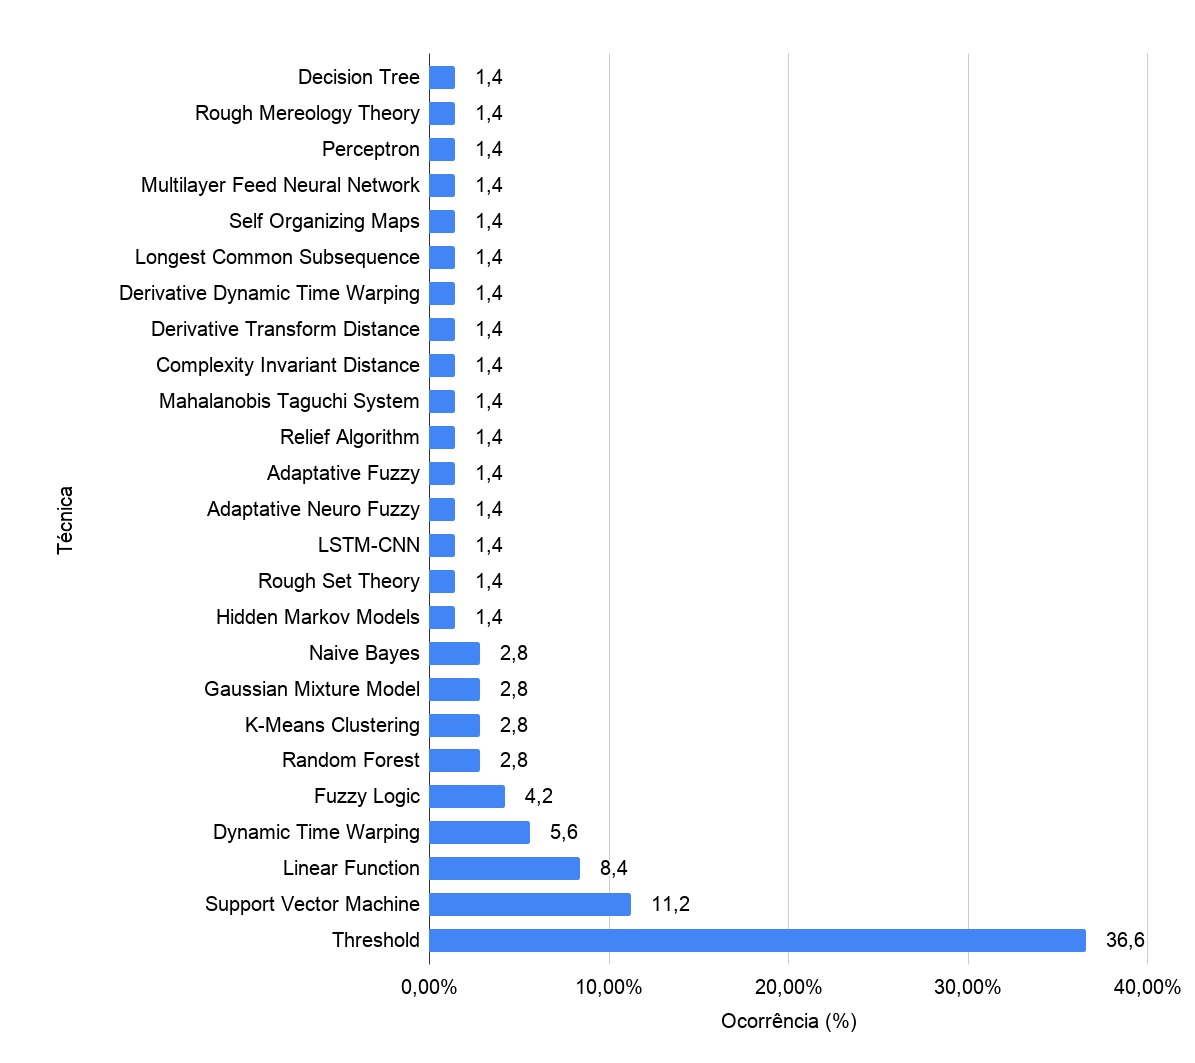
\includegraphics[width=0.95\textwidth]{figuras/fig_19.png}
    \fonte{Desenvolvido pelo autor.}
\end{figure}

\subsubsection{Abordagens Baseadas em Limiares} 

Os métodos baseados em limiares (\textit{threshold}) são extremamente simples e consistem na técnica mais utilizada nos estudos revisados. Esta abordagem é baseada na comparação dos valores pré-processados dos sensores com limiares estáticos ou dinâmicos. Alguns trabalhos utilizaram de mais de um valor de comparação, construindo assim uma heurística baseada em limiares. Esses valores de comparação, em geral, são obtidos por meio de análises exploratórias dos sinais dos sensores inerciais, sem muito rigor metodológico.

Na aplicação de limiares para o reconhecimento de exterocepção, foram identificados eventos transientes e persistentes. No estudo de \cite{Orhan2013} e \cite{Strutu2013} foram identificados buracos e redutores de velocidade. \cite{Akhtar2014}, \cite{Astarita2014}, \cite{Kaur2017} e \cite{Vittorio2014} reconheceram irregularidades do pavimento de forma genérica, sem classificar os padrões. \cite{Jamakhandi2014} detectou lombadas, poças e elevações abruptas. \cite{BelloSalau2018}, \cite{Gunawan2015}, \cite{Ghadge2015}, \cite{Kumar2017}, \cite{Li2018}, \cite{Pooja2017} e \cite{Rishiwal2016} identificaram solavancos/saliências e buracos, com \cite{Ghadge2015} validando o limiar com KMC e \textit{Random Forest}. \cite{Gawad2016} treinou um \textit{Perceptron} para gerar o limiar, posteriormente empregado na identificação de anomalias nas estradas. \cite{Afrin2015} identificou redutores de velocidade. \cite{Hsu2016} reconheceu buracos e identificou a qualidade da estrada, classificando em irregular, áspera ou lisa. \cite{Lima2016} classificou a qualidade do pavimento em boa, normal, ruim e péssima, enquanto \cite{Li2018} classificou em excelente/boa, regular, ruim, muito ruim/terrível.

Com relação à propriocepção, \cite{Niskanen2015} usou uma abordagem de limiares para medir o contato do pneu com a pista e com água e, então, detectou aquaplanagem. \cite{Matilainen2015} através o contato do pneu identificou a pista entre estradas secas e molhadas, informações úteis para o reconhecimento de aquaplanagem. \cite{Hou2017} detectou derrapagem. \cite{Sharma2015} identificou acelerações ou frenagens abruptas, curvas fechadas e mudanças de faixa frequentes. \cite{Li2016} detectou aceleração ou desaceleração anormal. \cite{Andria2016} identificou mudança de marcha: troca para marcha maior (suave ou forte) e redução de marcha (frenagem hidráulica ou frenagem com motor), além do estilo de direção: direção moderada ou agressiva. Finalmente, \cite{Gavruta2018} identificou curvas, acelerações e frenagens. 

\subsubsection{Abordagens de Alinhamento de Séries Temporais} 

Outra abordagem amplamente utilizada nos artigos foram as técnicas de alinhamento de séries temporais. Nessa abordagem, os estudos visam encontrar o alinhamento ótimo entre duas sequências de valores dependentes do tempo \cite{Muller2007}, para verificar a similaridade. Assim, dada uma série temporal que define um padrão de percepção, essa série é alinhada com os valores atuais do sensor para tentar reconhecer o padrão novamente. Na exterocepção, \cite{Alqudah2016} utilizou a técnica \textit{Dynamic Time Warping} (DTW) para detectar anomalias na pista. \cite{Singh2017} usou a mesma técnica para reconhecer buracos e solavancos/saliências. \cite{Souza2018} utilizou as técnicas DTW, \textit{Longest Common Subsequence Similarity} (LCSS), \textit{Derivative Dynamic Time Warping} (DDDTW), \textit{Derivative Transform Distance} (DTD) e \textit{Complexity Invariant Distance} (CID) para estabelecer a regularidade do pavimento asfáltico: regular ou deteriorado; tipo de superfície: asfalto, paralelepípedo e estradas de terra; e obstáculos no asfalto: lombada, remendo vertical, marcadores de elevação no pavimento e faixa de pedestres elevada. Na propriocepção, \cite{Pholprasit2015} utilizou o DTW para reconhecer frenagem, aceleração, virando à esquerda ou à direita, mudança de faixa à esquerda e à direita, além do perfil de direção classificado em não agressivo e agressivo.

\subsubsection{Abordagens de Funções Lineares}

As abordagens de função linear que identificamos visam mapear os padrões de vibração em índices de qualidade de estradas ou mapear eventos de condução em perfis de comportamento de direção. \cite{Prapulla2017} e \cite{BelloSalau2018} estabeleceram um índice personalizado de qualidade sobre a condição da pista. \cite{Brunauer2016} criou um índice de qualidade \textit{Road Surface Condition Index} (RSCI). \cite{Chen2013}, \cite{Douangphachanh2013}, \cite{Douangphachanh2014}, \cite{Li2018}, \cite{Pitonak2016}, \cite{Singh2017} e \cite{Tomiyama2016} mediram o Índice Internacional de Rugosidade (\textit{International Roughness Index} - IRI). Em \cite{Chen2013} foi calculado um índice de qualidade chamado \textit{Riding Quality Index} (RQI). Por meio do RQI, os valores foram mapeados para os conceitos de irregularidade, sendo eles: excelente, bom/competente e não competente. \cite{Saiprasert2014} mapeou eventos de direção para identificar o perfil de comportamento do motorista como muito seguro, seguro, agressivo ou muito agressivo.

\subsubsection{Outras Abordagens}

Os demais trabalhos analisados propuseram um conjunto amplamente variado de abordagens, desde de técnicas de caixa branca com inserção de conhecimento especializado até abordagens de caixa preta que empregam aprendizado de máquina. Na produção de exterocepção, \cite{Jang2015} usou uma \textit{Multilayer Feed Forward Neural Network} para classificar a estrada em classe de abrupta, irregular ou regular/suave. Em \cite{Selmanaj2014} foi utilizado de \textit{Self Organizing Maps} (SOM) para classificar a estrada em \textit{baseline}, irregular ou perigosa. \cite{Khaleghian2017} aplicou \textit{Fuzzy Logic} para reconhecer o tipo de superfície em grama, terra, concreto ou asfalto. \cite{Fouad2014} usou \textit{Rough Mereology Theory} para identificar redutores de velocidade. \cite{Allouch2017} utilizou \textit{Decision Trees}, SVM e \textit{Naive Bayes}, e \cite{Singh2018} usou uma SVM, ambos para identificar as condições da estrada de forma genérica. \cite{Nalavde2015} aplicou KMC e SVM para classificar a estrada em acidentada ou suave. \cite{Savera2016} usou SVM para detectar lombadas e valas, enquanto \cite{Gueta2017} com a mesma técnica identificou afundamentos, remendos, solavancos/saliências e buracos. \cite{El-Wakeel2018} usou SVM para reconhecer estradas suaves, buracos leves ou severos, bueiros leves ou severos, rachaduras transversais ou longitudinais, cavidades leves ou severas, faixas de desaceleração, lombadas, travessia ferroviária leve ou severa e estradas de paralelepípedo. Em \cite{M.2017} um \textit{Gaussian Model} identificou buracos e lombadas. \cite{Wang2018} aplicou o \textit{Mahalanobis Taguchi System} para identificar a tampa de bueiro, buracos e redutores de velocidade. \cite{Wickramarathne2018} através de \textit{Relief Algorithm} detectou buracos, solavancos e rachaduras.

Com relação à propriocepção, \cite{Wu2013} reconheceu os eventos de direção como direção normal, aceleração, desaceleração, mudança para as pistas da esquerda ou direita, direção em zigue-zague e aproximação do carro na frente através de \textit{Hidden Markov
Models}. Através de um sistema \textit{Fuzzy Logic}, também foi estabelecido um indicador de nível de perigo em relação à condução. \cite{Choudhary2014} também usou \textit{Fuzzy Logic} para identificar comportamento de direção perigoso. \cite{Arroyo2016} usou um classificador \textit{Adaptive Fuzzy} para identificar aceleração e frenagem. \cite{Eftekhari2018} aplicou \textit{Adaptive Neuro Fuzzy Inference System} para classificar a direção em segura, semi-agressiva ou agressiva. \cite{Bose2018} detectou frenagem e aceleração empregando um classificador \textit{Random Forest}. \cite{Vlahogianni2017} usou \textit{Rough Set Theory} para identificar aceleração, curvas à esquerda e à direita. \cite{Wu2018} aplicou \textit{Naïve Bayes} para classificar os eventos de direção em frenagem repentina, mudança casual de faixa, curva rápida, retorno rápido e estacionamento prolongado. \cite{Mahboob2017} usou um SVM para identificar curva à esquerda ou à direita, curva em U (meia-volta), frenagem abrupta ou suave. Finalmente, \cite{Saleh2017} aplicou uma LSTM-CNN para classificar o comportamento de direção em direção normal, agressiva ou motorista sonolento.

\subsection{Padrões de Percepção Veicular}

Vários tipos de dados de percepção foram identificados pelos estudos analisados nesta revisão. Além da classificação entre a exterocepção e a propriocepção, as percepções também foram classificadas quanto ao momento de detecção, sendo eventos transientes aqueles detectados momentaneamente, e eventos persistentes aqueles que ocorrem a todo o momento. 
Sendo assim, na exterocepção, são considerados eventos transientes obstáculos na estrada e anomalias de superfície, e eventos persistentes a identificação do tipo de pavimento, os índices de irregularidade e os níveis de qualidade. Na propriocepção, eventos transientes são eventos de condução e eventos persistentes são relacionados ao perfil do comportamento de condução. 
As figuras \ref{fig:exteroperception_occurrence} e \ref{fig:proprioception_occurrence} detalham as percepções encontradas.

\begin{figure}[h!]
  \centering
  \caption{Exterocepções encontradas nos estudos analisados}
   \label{fig:exteroperception_occurrence}
   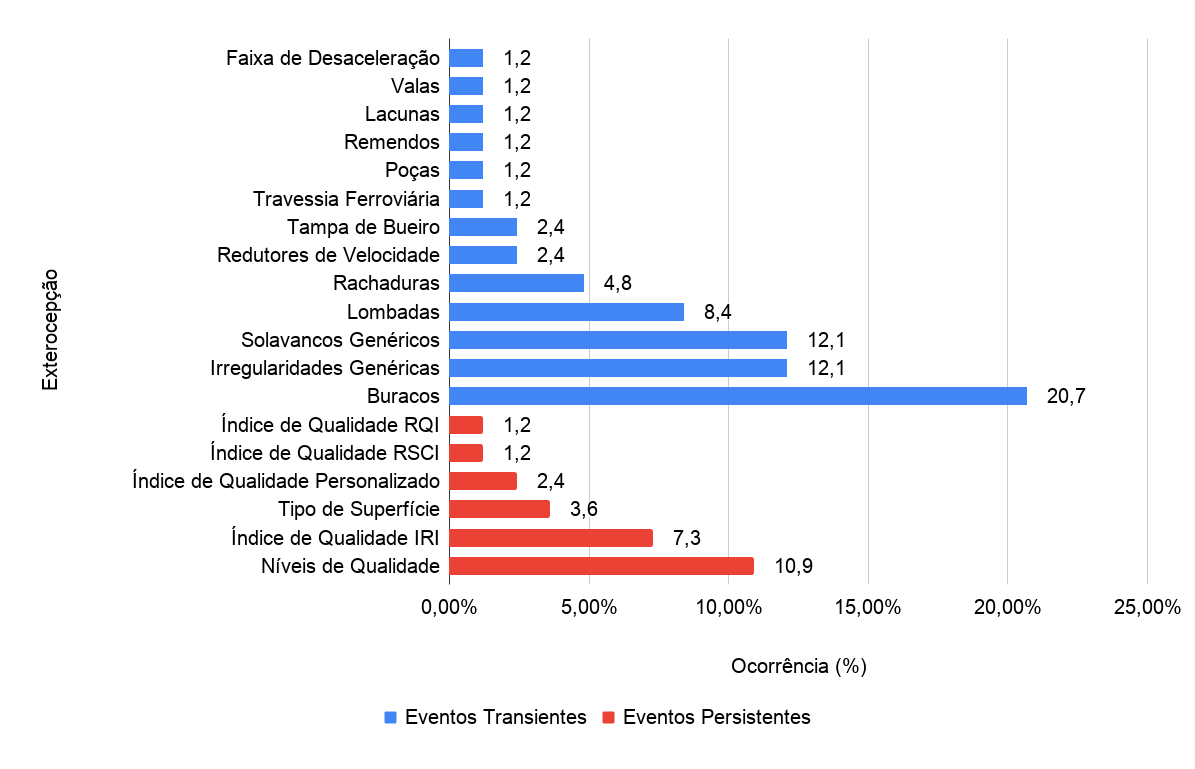
\includegraphics[width=0.95\textwidth]{figuras/fig_20.png}
    \fonte{Desenvolvido pelo autor.}
\end{figure}

\begin{figure}[h!]
  \centering
  \caption{Propriocepções encontradas nos estudos analisados}
   \label{fig:proprioception_occurrence}
   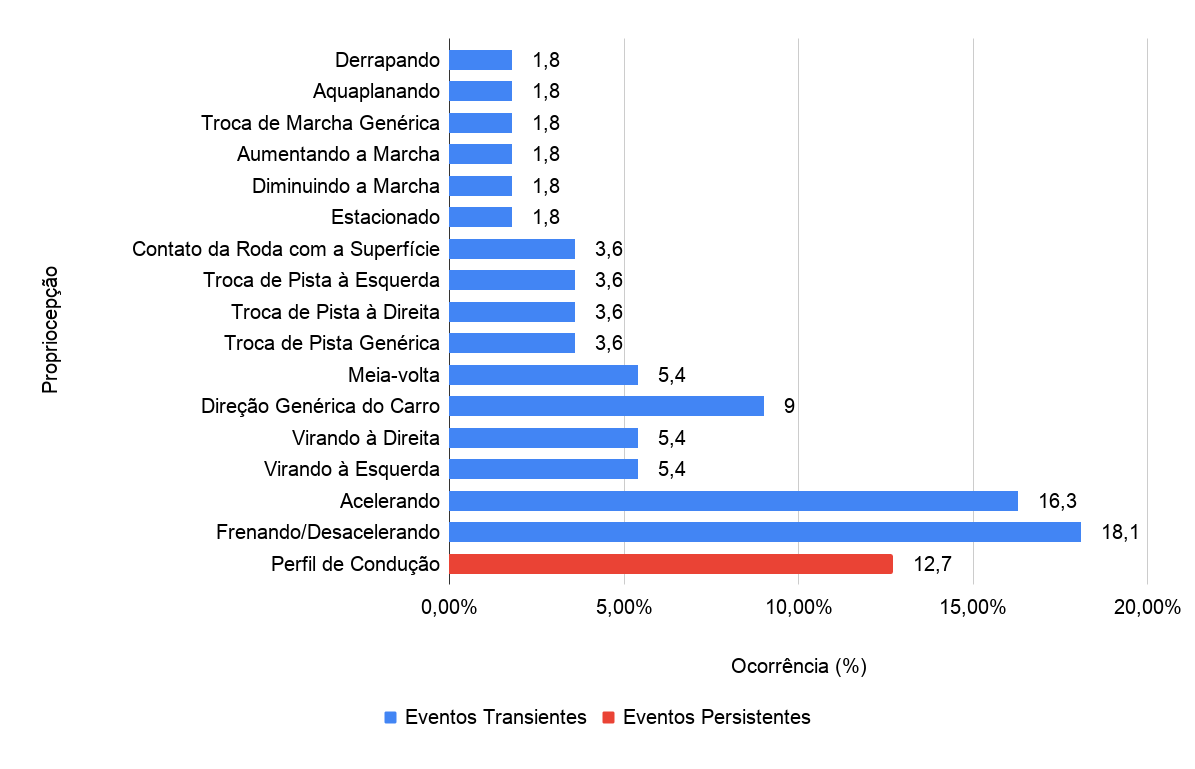
\includegraphics[width=0.95\textwidth]{figuras/fig_21.png}
   \fonte{Desenvolvido pelo autor.}
\end{figure}

\subsection{Áreas de Aplicação}

Alguns dos estudos analisados nesta revisão utilizaram as percepções percepções veiculares desenvolvidas em uma aplicação final. Os trabalhos que utilizam sensores embarcados em dispositivos móveis, devido a produzirem dados com menor confiabilidade, geralmente são aplicados em soluções de \textit{mobile crowdsourcing} com sensoriamento oportunista \cite{Afrin2015,Ghadge2015,Kaur2017,Kumar2017,Li2018,Lima2016,Pooja2017,Rishiwal2016,Savera2016,Singh2017, Strutu2013,Vittorio2014}. Neste tipo de aplicação, as soluções georreferenciam os eventos de percepção, enviando-os para um servidor central. Neste servidor, uma etapa de pós-processamento é aplicada, onde dados de diferentes fontes são integrados para melhorar a confiabilidade, como em \cite{Gawad2016} e \cite{Pooja2017}. Posteriormente, esses dados são disponibilizados de volta aos usuários em aplicativos como o ADAS \cite{Afrin2015,Akhtar2014,Nalavde2015}.

No uso de sensores inerciais fixados no veículo, os dados foram geralmente utilizados localmente. Em \cite{Selmanaj2014}, as percepções foram integradas ao desenvolvimento de um \textit{airbag}. Em \cite{Tomiyama2016} foi desenvolvido um sistema de monitoramento das condições da pista. \cite{Pitonak2016} buscou realizar controle de qualidade e garantia de qualidade no processo de entrega de projetos de engenharia civil. \cite{Khaleghian2017} utilizou do reconhecimento do tipo de superfície de pista para controlar a velocidade do veículo.

\subsection{Discussão e Conclusões}

Nesta revisão, foram analisados estudos publicados nos últimos sete anos que visam produzir padrões de percepção veicular por meio de análise multivariada de sinais de sensores inerciais. Os métodos revisados produzem vários padrões de eventos transientes e persistentes relacionados a exterocepção e a propriocepção. Constituindo uma abordagem não-intrusiva e passiva aplicada a um objeto em movimento, esses métodos permitem o monitoramento da infraestrutura de transporte e de seus participantes. Dado suas características de serem seguros, não poluentes, de fácil instalação e de baixo custo, esses métodos se mostram muito úteis quando empregados de forma ampla, com um grande número de usuários. Nesta seção, são comparados e discutidos vários aspectos dos métodos desenvolvidos nos artigos analisados. A discussão está estruturada de acordo com as etapas revisadas, sendo elas a coleta de dados, pré-processamento e processamento. Em seguida, são discutidos aspectos que envolvem todo o processo de reconhecimento e classificação dos padrões de percepção veicular, bem como sua aplicação nos mais diversos domínios.

Na primeira etapa, a coleta de dados foi realizada em contextos muito diferentes, com cada estudo amostrando sinais por meio de um determinado tipo de sensor, em uma plataforma específica, viajando em um determinado tipo de pavimentação, modelo de veículo e diferentes modos de condução. Assim, não foi encontrada uma metodologia comum para seleção de sensores, taxa de amostragem, colocação dos sensores na estrutura do veículo e seu posicionamento em relação aos referenciais. Desta forma, várias lacunas foram identificadas. Em relação aos sensores utilizados, a maioria dos estudos utilizou apenas o acelerômetro, ao invés de aplicar o giroscópio ou ambos. Essa seleção não se deve a critérios de qualidade, mas ocorre porque o acelerômetro é mais facilmente encontrado em dispositivos móveis, nos quais se concentra a maioria dos estudos. Porém, é necessário avaliar qual sensor fornece os melhores dados para gerar as percepções, e se a combinação dos dados de ambos pode melhorar os resultados dos modelos propostos.

Em relação às configurações de amostragem, os artigos revisados não discutem a faixa de medição utilizada, não deixando claro a possibilidade de saturação dos dados do sinal. Da mesma forma, poucos estudos justificam a escolha da taxa de amostragem, e os que o fazem definem este valor de acordo com limitações de processamento e economia de recursos da plataforma utilizada, não levando em consideração que em altas velocidades certos eventos podem não ser amostrados nas taxas estabelecidas. Assim, dada a grande quantidade de percepções veiculares que podem ser produzidas, é necessário estabelecer taxas de amostragem consistentes e não arbitrárias, permitindo a identificação das percepções de forma eficaz e eficiente, utilizando o mínimo de recursos computacionais necessários. No contexto de aplicação dos sensores inerciais em ITS é produzido valores grandes de aceleração e de taxa de rotação, de forma que o valor do erro agregado à resolução é insignificante e pode ser desprezado.

A colocação do sensor na estrutura do veículo ocorreu de várias formas, interna ou externamente à cabine. Uma vez que existem fatores de dependência relacionados às propriedades veiculares, a amostragem de dados em diferentes localizações no veículo implica em diferentes valores observados para um mesmo evento. Não foram encontrados estudos que correlacionassem sinais em diferentes partes do veículo para verificar uma possível variação na confiabilidade do reconhecimento devido a colocação do sensor. Também não houve estudos utilizando dados em mais de uma extremidade do eixo do veículo para analisar a possível melhoria nos resultados. O posicionamento dos sensores em relação aos referenciais tem sido abordado por poucos estudos, dificultando o entendimento de como os dados foram adquiridos e analisados. Finalmente, a maior lacuna nesta etapa se dá em razão da não existência de conjuntos de dados públicos desses sensores, para que se possa conduzir novas pesquisas ou comparar os métodos já propostos. Além disso, para que estes conjuntos sejam de fato úteis, é necessário que se siga toda uma metodologia de colocação na estrutura do veículo e posicionamento dos sensores de acordo com os referenciais.

Os dados foram amostrados por meio de duas plataformas, utilizando sensores embarcados em dispositivos móveis, como \textit{smartphones} e \textit{tablets}, ou anexados à estrutura veicular, empregando microcontroladores ou SBC. Na primeira plataforma os dados são menos confiáveis do que na segunda, uma vez que os sensores não permanecem fixos o tempo todo e não possuem uma colocação e posicionamento predefinidos. Isso implica que não há garantia de padronização do referencial de análise, ou seja, a localização dos eixos dos sensores podem variar constantemente em relação aos do veículo. Desta forma, não foram encontrados métodos aplicados localmente para garantir a qualidade dos dados amostrados em dispositivos móveis, considerando a possível interferência nestes dispositivos, principalmente humana. Alguns métodos voltados a prover maior confiabilidade dos dados foram empregados em servidores centrais que recebem padrões reconhecidos de várias fontes. No entanto, eles não se mostram úteis se as fontes primárias sempre fornecerem resultados insatisfatórios devido ao referencial incorreto. O único método que visa fornecer certa confiabilidade são as fórmulas para reorientação dos eixos baseadas nos ângulos de Euler, as quais possuem diversas limitações discutidas na etapa de pré-processamento, principalmente devido ao mapeamento dos eixos do sensor para o referencial do mundo real e não para o referencial do veículo. Nenhum dos estudos discute a comparação dos aspectos da coleta de dados nas duas plataformas apresentadas, e a possibilidade de se criar um modelo de reconhecimento de percepção possível de ser utilizado em ambas. Além dos sensores inerciais, alguns estudos utilizaram fontes de dados auxiliares. O GPS e OBD-II foram usados para obter a velocidade do veículo, a qual consiste de um dos fatores de dependência. Alguns estudos também utilizaram o sensor de magnetômetro para medir o campo geomagnético ambiental, que foi empregado com os dados de aceleração para calcular os ângulos de Euler durante a reorientação do eixos. 

Uma vez coletados, todos os dados brutos foram pré-processados antes de serem passados para a técnica que reconhece e classifica os padrões de percepção. O pré-processamento foi subdividido em três etapas de acordo com sua finalidade. Na primeira etapa de pré-processamento, foram aplicados métodos de reorientação dos eixos entre os referenciais do sensor e do veículo. Diretamente relacionados aos referenciais de coleta e análise, duas técnicas foram apresentadas para esse fim: posicionamento controlado e fórmulas baseadas em ângulos de Euler. No posicionamento controlado, aplicado na etapa de coleta de dados, embora os dados sejam amostrados em um referencial correto para análise, a técnica é suscetível a erros quando utilizada em sensores não fixados no veículo, como os embarcados em \textit{smartphones} e \textit{tablets}. Isto se deve ao possível desalinhamento dos eixos, ocasionado pela não fixação dos sensores. Em relação aos ângulos de Euler, as três formas apresentadas para o cálculo dos ângulos possuem limitações específicas. Na primeira, apresentada em \cite{Orhan2013,Vittorio2014,Singh2017}, devido ao uso de uma orientação inicial que não é atualizada continuamente, os valores em locais com aclive ou declive do terreno podem apresentar erros. Isso se deve ao fato de que nesses locais a força de aceleração gravitacional é distribuída entre os eixos, não ficando isolada no eixo de aceleração vertical. Na segunda técnica apresentada em \cite{Li2018}, embora os ângulos sejam atualizados, o valor da força gravitacional não é isolada e pode levar a erros por não ser o único componente de força presente nos eixos. Na terceira técnica de \cite{Singh2018}, devido à tentativa de identificar um possível estado estacionário durante a condução do veículo para defini-lo como um novo referencial inicial, isso implica que estradas de alta vibração não satisfazem as condições e não atualizam os ângulos, acumulando erros.

Todos os métodos apresentados de cálculo dos ângulos de Euler para reorientação do eixos são baseados na localização da força de aceleração gravitacional. Sendo assim, os ângulos de rotação devem sempre ser calculados a partir de um estado estacionário, e não em relação aos dados de aceleração atuais como feito em alguns estudos. As fórmulas matemáticas e as condições de aplicação podem ser encontradas no estudo primário \cite{Astarita2012}, que é referenciado e utilizado pelos artigos revisados. Ainda por serem baseadas na gravidade, as técnicas reorientam o eixo Z perpendicularmente ao solo, apontando para o céu, ao invés de ser perpendicular ao chão do veículo. Portanto, os dados são reorientados para o referencial do mundo real e não para o referencial do veículo, que apenas se sobrepõe ao eixo Z em casos de terreno plano. Essa técnica de reorientação somente é útil quando usada em dispositivos móveis com sistemas de \textit{mobile crowdsensing}, produzindo apenas exterocepção. Nos métodos de reorientação analisados, os eixos X e Y ficam sem uma orientação bem definida. Para a propriocepção, mesmo adicionando orientação ao eixo X e Y através do magnetômetro, o referencial do mundo real (terra) não permite identificar eventos de condução, sendo necessário estar no referencial do veículo. Convém frisar que os métodos apenas são aplicáveis a reorientação dos dados de aceleração, e não para os de taxa de rotação. Portanto, a abordagem do posicionamento controlado, embora simples, com o fixação de sensores e alinhamento dos eixos apresenta menor possibilidade de erros, permitindo reconhecer a exterocepção e a propriocepção.

Na segunda etapa de pré-processamento, pré-processamento de sinal, foram aplicados métodos para remoção de ruídos, suavização de sinal, segmentação de dados e extração de características. Em resumo, os estudos aplicaram métodos estatísticos no domínio do tempo, e métodos como transformadas e \textit{wavelets} no domínio da frequência. No domínio do tempo, métodos como médias simples ou móveis foram aplicadas para remover ruídos e suavizar os sinais. Métodos como o desvio padrão e o RMS foram aplicados para extrair características de alto nível que bem representassem os dados para o reconhecimento de padrões. No domínio da frequência, métodos como IIR e \textit{Butterworth} foram utilizados para remover ruído, através de frequências específicas, como a da gravidade nos dados de aceleração. A FFT e as \textit{wavelets} foram empregadas para extrair características tais como magnitudes das vibrações. Não encontramos uma análise comparativa dos métodos de remoção de ruído e extração de características em seus diferentes domínios, sendo uma lacuna a ser explorada. Em relação ao domínio de processamento, a maioria dos métodos foi aplicada no domínio do tempo, sendo que os domínios da frequência e do tempo-frequência devem ser melhor explorados, para se verificar a possibilidade de produzir dados mais relevantes para as técnicas de classificação. A segmentação dos dados foi realizada de quatro formas: em função do tempo, número de amostras, distância ou velocidade. Em geral, o uso da janela em função da distância é mais adequado. Não encontramos nos estudos analisados um valor ideal para o tamanho da janela de dados. Em pesquisas futuras, o impacto do valor deste parâmetro deve ser avaliado.

Na terceira etapa do pré-processamento, foram aplicados os métodos de georreferenciamento dos dados. Uma vez que a taxa de amostragem de dados de sensores inerciais é muito maior do que a de dados de localização (1 Hz), são necessárias técnicas para estimar a localização (posição mais granulada) e a velocidade, antes da próxima amostra de GPS. Para fazer isso, apenas \cite{Li2018} utilizou um tratamento, aplicando interpolação linear com os dados de aceleração para obter dados de localização com mais frequência. Porém, o mesmo não foi feito com a velocidade. O desenvolvimento de um método para esse fim é de extrema importância, uma vez que a velocidade constitui um fator de dependência e deve ser o mais próximo possível do real. Da mesma forma, estimar pontos de localização ajuda a mitigar pontos cegos, reduzir o erro de localização, entre outros problemas. Não identificamos nenhuma desvantagem em usar este método, exceto o aumento do processamento do modelo.

Na etapa de processamento, várias técnicas foram propostas para reconhecer e classificar os padrões nos dados pré-processados dos sensores. Embora alguns trabalhos apresentem técnicas com abordagens mais elaboradas, como métodos de alinhamento de séries temporais, aprendizado de máquina e modelos com conhecimento especializado, quase metade deles utiliza de técnicas extremamente simples, como limiares e funções lineares. As demais técnicas empregadas são geralmente clássicas, sendo necessário testar e avaliar técnicas mais recentes. Dentre as abordagens mais recentes, o \textit{Deep Learning} é um dos que apresenta o maior potencial para melhorar os resultados de reconhecimento e classificação das percepções veiculares, o qual nos últimos anos fez grandes avanços nos mais variados domínios \cite{LeCun2015}. Uma das grandes vantagens das técnicas de \textit{Deep Learning} está em adicionar a segunda etapa de pré-processamento ao modelo de treinamento. Dessa forma, o melhor método para remover ruído e extrair recursos de alto nível dos dados brutos é definido por meio do treinamento. Nos estudos analisados, essa abordagem foi encontrada em apenas uma pesquisa \cite{Saleh2017}, que se limita a um tipo específico de percepção. Portanto, é uma abordagem que deve ser mais explorada nesta área de pesquisa.

Em relação às variáveis de entrada utilizadas pelas técnicas, a maioria dos estudos utilizou apenas dados do eixo em que as percepções são mais evidentes. Assim, analisando no referencial do veículo, os padrões de exterocepção são mais evidentes na aceleração do eixo Z e nas taxas de rotação dos eixos X e Y. Já os padrões de propriocepção são mais evidentes nos dados de aceleração dos eixos X e Y e na taxa de rotação do eixo Z. Contudo, embora não visualmente evidentes, as percepções também produzem dados significativos nos demais eixos, conforme discutido em \cite{M.2017}. Portanto, é importante considerar todos os eixos dos sensores inerciais no reconhecimento de percepção, bem como a velocidade do veículo. Além disso, os estudos geralmente se concentram no reconhecimento de uma percepção específica, não trabalhando a correlação e integração de diferentes tipos de percepção, bem como na integração entre a exterocepção e a propriocepção. Essa integração se deve ao fato de que várias percepções são dependentes ou correlacionadas entre si. Um exemplo de dependência ocorre no reconhecimento do tipo de composição da superfície da estrada que depende da ausência de derrapagem ou aquaplanagem. Quanto à correlação, em geral a percepção de desaceleração por frenagem está relacionada a algum obstáculo, como buraco ou lombada. Adicionar essas percepções como variáveis de entrada para o reconhecimento de outras pode melhorar os modelos. 

Os resultados dos métodos propostos não foram comparados nesta revisão por vários motivos. Em primeiro lugar, a maioria dos estudos não tem resultados medidos ou métricas semelhantes para comparação. A metodologia aplicada também não é clara em muitos deles, carecendo de muitas informações relevantes. Além disso, cada trabalho foca em algum tipo específico de percepção, não permitindo a comparação direta devido aos diferentes propósitos dos métodos. Por fim, a maior limitação para a não comparação se deve ao fato de os dados serem amostrados em contextos significativamente distintos, conforme detalhado anteriormente, fazendo com que as comparações tornem-se subjetivas, principalmente pela existência de fatores de dependência. Da mesma forma, a ausência de conjuntos de dados públicos impossibilitou a realização de testes de avaliação dos métodos. Assim, esta revisão teve como foco a análise de aspectos dos métodos e técnicas aplicados em todas as etapas da coleta e análise de dados.

Através da análise dos estudos, foi observado um enfoque maior na simples e imediata aplicabilidade dos resultados do que em fornecer dados mais precisos e acurados com uma certa adaptabilidade. Isso mostra-se mais evidente em aplicações de sensores embarcados em dispositivos móveis. Sendo assim, a maioria dos trabalhos foca na aplicação das percepções produzidas, e a adaptabilidade das soluções apresentadas é pequena, sendo o principal obstáculo para sua ampla utilização em cenários do mundo real. Em relação aos fatores de dependência, a adaptabilidade raramente é mencionada nos artigos. Alguns estudos adicionaram em seus modelos o fator de velocidade ou o modelo \textit{Quarter Car} (QC) \cite{Tomiyama2016}, porém nenhum deles trata de todos os fatores de dependência para produzir diferentes tipos de percepção. Além disso, nenhum dos estudos experimenta o modelo \textit{Half-Car} (HC), que pode ser mais interessante em aplicações de \textit{mobile crowdsensing} que o QC. \cite{Singh2017} argumenta que não é possível cobrir todas as condições por meio de aprendizado de máquina e modelos de limiares existentes. No entanto, a adaptabilidade deve ser investigada do ponto de vista das três etapas apresentadas, especialmente integrando os dados com as novas técnicas robustas de aprendizado de máquina. Outro ponto a ser explorado no sentido de adaptabilidade e ainda não observado nos estudos é a integração dos dados de percepção, conforme mencionado anteriormente. Por exemplo, eventos persistentes que descrevem as condições gerais da pista de um determinado segmento de estrada podem ser considerados como fatores de dependência: o tipo de composição e o estado de conservação da superfície implicam em padrões diferentes para o mesmo evento transiente. Assim, um buraco detectado no pavimento asfáltico pode ter um padrão diferente de buracos em outros tipos de pavimento. Isso também deve ser levado em consideração por abordagens adaptativas.
 
Em relação ao tempo de detecção, os estudos produziram as percepções de forma \textit{offline}, \textit{online} e em tempo real. No entanto, a maioria deles confunde os termos \textit{online} e tempo real, havendo necessidade de em novos estudos analisar restrições temporais de resposta dos modelos. Em relação à aplicação, nos estudos analisados, os dados de percepção veiculares foram utilizadas principalmente em ADAS. Porém, por consistir em um segmento dentro de ITS, novas aplicações podem se beneficiar dessas identificações como caixa preta veicular para seguradoras, sistemas de informações situacionais de planejamento de manutenção de estradas ou aplicados a agentes inteligentes para navegação autônoma. Além disso, embora uma ampla gama de percepções possa ser observada nos estudos, identificamos situações onde é possível criar novas percepções a partir dos sensores inerciais, tais como a identificação de relevo.

\section{Análise de Percepções Veiculares Específicas}

Nesta seção, embasado no estado da arte levantado pela revisão da literatura, é discorrida uma análise comparativa dos aspectos mais relevantes dos trabalhos relacionados  as três percepções abordadas nesta pesquisa. Nas seções subsequentes são analisados, respectivamente, os trabalhos de classificação de tipo de superfície de pista, de qualidade de superfície e de reconhecimento de lombadas.

\subsection{Classificação do Tipo de Superfície de Pista}

Baseando-se nas propriedades de dependência apresentadas, analisamos os modelos propostos em pesquisas relacionadas a fim de verificar quais propriedades foram adotadas. Os estudos para classificação de tipo de superfície com sensoriamento inercial encontrados foram conduzidos em dois tipos de veículos: \textit{wheeled ground robots} \cite{Khaleghian2017, Sebastian2019, Tolentino-Rabelo2016} e carros \cite{Souza2018, Wang2018_1, Wang2017}. Uma vez que a estrutura entre os dois tipos de veículos é muito diferente, e existe a propriedade de dependência veicular, os trabalhos de \textit{wheeled ground robots} não foram considerados. Dentre os estudos que aplicam os sensores em carros, \cite{Souza2018} utilizou sensores embarcados em \textit{smartphones} e \cite{Wang2018_1, Wang2017} fixaram no veículo. 

Em \cite{Souza2018} o \textit{smartphone} com sensores foi fixado dentro do veículo usando um suporte de sucção flexível perto do painel. O modelo desenvolvido utilizou de dados do acelerômetro (100 Hz) e velocidade do GPS, obtendo os melhores resultados com o modelo de LCSS combinado com CID. Como resultado, a superfície de pista é classificada entre asfalto (98.28\%), paralelepípedo (84.41\%) e terra (78.64\%), obtendo na média 87.77\% de precisão. Em  \cite{Wang2018_1} e \cite{Wang2017} foi utilizado dados do acelerômetro montado na suspensão veicular e velocidade do GPS. No pré-processamento foi empregado o modelo matemático QC, de forma a considerar a influência da suspensão veicular, e FFT para extração de características. Estes dados foram treinados em uma SVM, classificando a pista em asfalto (17.6\%), concreto (99.6\%), grama (74.9\%) e terra (85.3\%), com média de precisão de 69.4\%. 

Analisando os estudos, observamos que são limitados ao uso de dados de aceleração, velocidade e modelo QC. Sendo assim, não são exploradas todas as propriedades de dependência e não é analisado o comportamento do modelo em variações contextuais. O ambiente de coleta não é detalhado de forma adequada, de forma não ser possível verificar condições de conservação dos pavimentos ou presença de irregularidades e obstáculos. Também não há especificação dos veículos utilizados e seus condutores, e se foram utilizados mais de um. Por fim, os resultados obtidos apresentam baixos valores das métricas de avaliação, mesmo em cenários controlados.

\subsection{Classificação da Qualidade de Superfície de Pista}

Baseado no estado da arte e nos aspectos relevantes levantados, como os fatores de dependência, analisamos os modelos propostos em pesquisas relacionadas para verificar quais propriedades foram levadas em consideração. Para classificação da qualidade da superfície de pista, os estudos se concentraram na criação de índices de irregularidade e níveis de qualidade. Os trabalhos correlatos empregaram sensores em \textit{smartphones} \cite{Douangphachanh2014_1,Lima2016,Brunauer2016,Zhao2016,Allouch2017,Souza2018_1,Li2018,Nunes2019,Tiwari2020,Badurowicz2020,AbdelRaheem2020} e fixados em veículos \cite{Chen2013, Chen2016,Pitonak2016,Prapulla2017,Pont2017,Lei2018,Hassan2019,AbdelRaheem2020,Monica2021}.

Em \cite{Nunes2019} foi apresentado um \textit{framework} para classificar a qualidade de uma estrada entre boa e ruim, experimentado em vias urbanas. Para isto, um aplicativo coleta localização e velocidade através do GPS, além de dados do acelerômetro, ambos embarcados em \textit{smartphones}. Junto com os dados, o dispositivo coleta a opinião do usuário sobre a via, para utilizar como rótulo das classes de dados. Os dados coletados são enviados para um servidor na nuvem, que pré-processa os dados, empregando com modelos de \textit{Random Forest}, KNN, J48 e SVM, os quais obtiveram acurácia respectiva de 90.64\%, 86.04\%, 75.67\% e 74.97\%. Em \cite{Douangphachanh2014_1} foi realizado experimentos para analisar a relação entre as frequências dos dados de aceleração e os níveis de irregularidade da via. Neste estudo, foram coletados dados de acelerômetro (100 Hz) e GPS embarcados em \textit{smartphones}. Os dispositivos foram colocados em diferentes locais, como bolso da camisa do motorista e próximo ao câmbio de marchas, e em diferentes veículos. Com os dados coletados, foi realizado uma análise no domínio da frequência através da aplicação de FFT, para verificar a relação entre a magnitude das frequências e as classes de dados de qualidade da via: boa, regular, ruim e péssima.

Em \cite{Souza2018_1} foi proposto um sistema para monitorar as condições do pavimento. Para isto, utilizaram de um \textit{smartphone} com sensores foi fixado dentro do veículo usando um suporte de sucção flexível perto do painel. O modelo desenvolvido utilizou de dados do acelerômetro (100 Hz) e velocidade do GPS. Através dos dados coletados, foram extraídas características no domínio do tempo, com métodos estatísticos, e na frequência, com FFT, aplicadas em SVM, \textit{Random Forests}, \textit{Naive Bayes}, \textit{Decision Trees}, e KNN. O modelo de SVM apresentou os melhores resultados, classificando com 92,39\% de acurácia os segmentos entre bom, regular, ruim, péssimo e trecho com obstáculos. As classes de dados foram anotadas a partir da percepção de pessoas. \cite{Tiwari2020} utilizaram de acelerômetros em \textit{smartphones} para classificar a via entre boa, mediana e ruim. O GT foi feito de forma humana, através da observação das gravações de câmeras. Os dados foram coletados em ambiente urbano, somente em vias pavimentadas, sumariamente asfalto. Através dos dados de aceleração, foram extraídas características por meio de métodos estatísticos. Estas características foram aplicadas em uma SVM, uma \textit{Feed-forward Neural Network} e uma CNN, as quais obtiveram respectivamente acurácia de 65.6\%, 65.7\%, e 98.5\%.

Em \cite{Badurowicz2020} foi desenvolvida uma heurística de limiares junto com um sistema \textit{Fuzzy Logic} para classificar a qualidade da via entre boa, medíocre e pobre. O estudo utiliza dos dados de um acelerômetro em \textit{smartphone}. \cite{Leizerovych2020} desenvolveram uma aplicação para análise da condição da via. Para isto foi utilizado de acelerômetro, giroscópio e GPS em \textit{smartphones}. Os dados coletados em vias de asfalto foram empregados em uma CNN para classificar a pista entre lista, satisfatória e insatisfatória. A acurácia do estudo foi de 84.81\%. \cite{Allouch2017} apresentaram modelos para classificar a qualidade da via. Para isto, foi utilizado de acelerômetro, giroscópio e GPS em \textit{smartphones}. No pré-processamento foi utilizado FFT para extração de características. Para classificar as vias entre normal e esburacada, as características foram aplicadas em \textit{Decision Tree}, SVM e \textit{Naive Bayes}, as quais obtiveram acurácia de 98.50\%, 95.25\% e 96.90\%, respectivamente.

Em \cite{Lima2016}  foi desenvolvida uma aplicação para estimar a qualidade da via, assim como problemas transientes no asfalto. Para isto, utilizaram de acelerômetro e GPS em \textit{smartphones}. Os dados de aceleração e velocidade foram empregados em uma heurística de limiares para classificar a via em boa, normal, ruim e péssima.
\cite{Brunauer2016} desenvolveram uma aplicação para calcular o RCSI. Para isso utilizaram de acelerômetro e GPS em \textit{smartphones}. Para calcular o RCSI, foi empregado uma função linear simples que mapeia a quantidade de eventos transientes detectados para cinco níveis de qualidade (1-5). \cite{AbdelRaheem2020} utilizaram GPS e acelerômetros fixados no veículo e em \textit{smartphones} para calcular o IRI. Os sensores foram utilizados em um único carro, em velocidade entre 30km/h e 40km/h. O estudo utilizou apenas a aceleração vertical na fórmula simplificada de calculo IRI. 

Em \cite{Li2018} foi apresentado um aplicativo de \textit{mobile crowdsensing} para analisar irregularidades na superfície da estrada. Para isso, utilizaram de um acelerômetro e GPS em \textit{smartphones}, fixados na cabine do veículo por meio de suporte. No acelerômetro, os sinais foram processados para reorientar os dados, com fórmulas baseadas nos ângulos de Euler. Posteriormente, usando os filtros passa-alta e passa-baixa, o componente de gravidade foi removido. Em segmentos de 50 metros foi calculado o índice IRI-proxy, através da normalização do RMS de aceleração vertical pela velocidade. \cite{Zhao2016} desenvolveram uma aplicação para calcular o IRI. Para isso utilizaram de acelerômetro e GPS em \textit{smartphones}, utilizado em três veículos e quatro diferentes locais de coleta, todos acima da suspensão. A velocidade empregada ficou entre 40km/h e 60km/h. Para calcular o IRI foi empregado os dados de aceleração vertical no modelo HC e fórmulas do IRI. Os parâmetros do modelo HC foram definidos por um algoritmo genético.

Em \cite{Chen2013} e \cite{Chen2016} foi desenvolvido um sistema de \textit{crowdsourcing} para monitoramento da superfície de pista. O estudo utiliza de um conjunto de \textit{hardware} fixado no veículo, composto por um acelerômetro (100 Hz), um GPS e um microcontrolador. O desvio padrão dos dados de aceleração são empregados em uma função linear simples para estabelecer o IRI. Posteriormente, outra função linear mapeia o IRI para o RQI, e deste para quatro níveis de qualidade: excelente, boa, qualificada e desqualificada. \cite{Lei2018} apresentaram uma plataforma para monitoramento de superfície da via. Neste estudo foi utilizado apenas a aceleração vertical amostrada em acelerômetros conectados à um microcontrolador. A plataforma foi fixada na entrada USB do veículo. Os rótulos das classes de dados foram estabelecidas com base na opinião de pessoas, classificando a qualidade da via em um índice \textit{Present Serviceability Rating} (PSR) de 0-5. Os dados de aceleração foram aplicados em uma FFT, onde foi analisado a relação entre as diferentes frequências e os níveis de qualidade.

Em \cite{Monica2021} desenvolveram uma abordagem para estabelecer dois indicies de irregularidade da via, assim como conceitos de qualidade relacionados. Para isto, o estudo utilizou de sensores inerciais (100 Hz) e GPS embarcados em caixas pretas veiculares. Os dados foram coletados em vias asfaltadas de área urbana, em velocidade de 30 km/h até 50 km/h. O método utilizou da aceleração vertical e velocidade coletadas em métodos estatísticos tais como média móvel e desvio padrão para estabelecer dois índices de irregularidade: \textit{Local Pave Box index} (LPBi) e \textit{Global Pave Box index}  (GPBi). Através de limiares, estes índices foram mapeados para níveis os qualidade bom, regular, ruim e trecho precisando de reparos. \cite{Pont2017} utilizaram de acelerômetros e GPS no veículo para avaliar o conforto de condução com base na qualidade da via. Através de uma função simples que tem como entrada a aceleração e velocidade, é estimado o RQI. Este índice é comparado com limiares para classificar a via entre crítica e não crítica.

Em \cite{Hassan2019} foi desenvolvido um método para classificação da qualidade de pista baseado na quantidade de obstáculos e irregularidades. Para isso, um acelerômetro e GPS foram instalados em veículos, e seus dados foram processados para identificar eventos como lombadas e buracos. De acordo com a quantidade de eventos encontrados, a via é classificada entre boa, regular, ruim e terrível. \cite{Prapulla2017} utilizaram um acelerômetro e GPS em um Arduíno. Nos dados de aceleração é empregado desvio padrão, valor utilizado para segmentar a qualidade da via. \cite{Pitonak2016} utilizou de um giroscópio instalado no veículo para calculo do índice IRI. Para isto, foi utilizado o valor \textit{pitch} em uma função linear. Posteriormente, o resultado da função é aplicado em outra função que mapeia para o IRI, através de correção.

Através da análise dos trabalhos relacionados, é possível observar que nenhum deles busca considerar todos os fatores de dependência. Alguns dos estudos consideram diferentes velocidades ou diferentes veículos, embora nenhum dos estudos considere todos os fatores em conjunto. Em relação aos ambientes, os estudos na sua grande maioria realizam a identificação de qualidade de pavimentos asfálticos, não analisando outros pavimentos ou a vias sem pavimentação. Os níveis de qualidade, em muitos casos, são simples mapeamentos de um índice personalizado de irregularidade para conceitos, não se mostrando confiáveis uma vez que os modelos que geram os índices são extremamente simplistas. Em relação à quantificação de irregularidade pelos mais variados índices, nota-se que estes indicadores são fortemente dependentes dos conjuntos de dados utilizados, isto porque os fatores de dependência não são levados em consideração, e sumariamente os índices consideram apenas a aceleração vertical no cálculo. 

Os índices em geral constituem de funções lineares simples de um componente apenas. No caso do IRI, embora suas fórmulas sejam robustas e considerem toda a mecânica veicular envolvida, os estudos utilizam das fórmulas reduzidas pela aplicação dos parâmetros \textit{Golden Car}, os quais padronizam diversos aspectos, tais como velocidade constante em 80 km/h. Estes parâmetros não são adequados para aplicação real justamente por se limitarem a um cenário específico, um determinado sistema de amortecimento, determinada velocidade, etc. Em aplicações do mundo real, estes valores possuem grande variação. Em relação a rotulação dos dados, praticamente todos utilizam de anotação manual de GT humano, tornando extremamente subjetivo o que pode ser classificado como bom ou ruim. Mostra-se necessário desenvolver um GT anotado por máquina para não haver diferentes percepções de qualidade em relação a um mesmo segmento de via. Em relação aos dados utilizados, muitos utilizam apenas de um eixo do sensor para fazer análise.  Diversos estudos relacionados se mostram prova de conceito, faltando detalhes do ambiente de coleta, colocações dos sensores, e métricas de resultados insuficientes para análise aprofundada.

\subsection{Reconhecimento de Lombadas}

Através dos estudos analisados, é possível observar que a grande maioria possuí foco na identificação de eventos em uma forma genérica, em classes de dados tais como \emph{obstáculo}, \emph{anomalia} ou \emph{irregularidade}. Considerando como exemplo buracos e lombadas, agrupá-los em um único identificador torna a aplicação de ITS menos inteligente, especialmente se considerarmos que um buraco é uma irregularidade que deve ser corrigida e deixar de existir, enquanto que a lombada é um obstáculo que sempre estará lá. Desta forma, a especificação da informação situacional durante a detecção se mostra importante, e nesta seção são analisados somente os estudos que realizam a identificação de lombadas como uma de suas classes de dados.

Para identificação de lombadas através de sinais de sensores inerciais, a coleta de dados ocorreu com a utilização destes dispositivos em duas formas: fixados no veículo \cite{Sabir2019,Padilla2018} ou embarcados em \textit{smartphones} \cite{Fouad2014,Alam2020,Rishiwal2016,Wang2018,Verma2016,Souza2018,Edwan2019,Savera2016,Idris2019,Dey2019,Aljaafreh2017,Aragon2016}. No trabalho de \cite{Rishiwal2016} foi desenvolvida uma aplicação para detecção de buracos e lombadas. Os dados foram coletados através de acelerômetro e GPS em um \textit{smartphone}. Para reconhecer os padrões foi utilizado de limiares condicionados por intervalos de velocidade. A acurácia da abordagem proposta foi de 93.75\%. Em \cite{Verma2016} foi desenvolvido uma aplicação para estimar o tempo de viagem utilizando de localização de lombadas, curvas e e paradas obrigatórias. Como fonte de dados, o estudo utilizou acelerômetro, giroscópio, bússola e GPS. Para detectar lombadas, foi utilizado de limiares com os valores de aceleração no eixo Z, obtendo acurácia de 87.5\%. Em \cite{Edwan2019} desenvolveram uma aplicação para dispositivos móveis que detecta e avisa lombadas na via. Foram utilizados acelerômetro e GPS em \textit{smartphones}. As lombadas foram reconhecidas através de limiares.

Em \cite{Savera2016} desenvolveram um aplicativo para detectar e alertar lombadas e buracos na pista. Para isto, foram utilizados sensores acelerômetro e GPS em \textit{smartphones}. Os dados foram coletados de diferentes dispositivos e em diferentes veículos. Posteriormente, os dados foram aplicados em uma SVM. Na detecção de lombadas o estudo obteve 86.34\% de acurácia, 90.80\% de precisão, 94.61\% de \textit{recall}, 92.67\% de \textit{f1-score}. \cite{Idris2019} desenvolveram uma aplicação para reconhecer buracos e lombadas. O estudo utilizou de dados de um acelerômetro embarcado em \textit{smartphone}. Os dados foram coletados em um mesmo segmento de via com diferentes veículos. Após coletados, foram os dados foram pré-processados em segmentos de desvio padrão aplicados em uma SVM. Em \cite{Dey2019} desenvolveram uma aplicação to condições da via, dentre as quais a identificação de lombadas. Para isto, utilizaram de acelerômetro e magnetômetro embarcados em \textit{smartphones} colocados em diferentes locais, como painel, suporte para copo e dentro do bolso. As análises foram feitas utilizando diversos algoritmos de classificação, como \textit{Random Forest}, \textit{Random Tree} e SVM.A classificação foi feita após a seleção de características usando os algoritmos \textit{GreedyStepwise}, \textit{Ranker} e \textit{BestFirst}, considerando o valor mínimo, máximo, mediana e desvio padrão como recursos estatísticos. O estudo obteve 92 \% de precisão para detectar as condições da superfície da estrada.

Em \cite{Aragon2016} desenvolveram um modelo para classificar diferentes tipos de anomalias presentes em estradas, como buracos e lombadas. Para isto, foram utilizados dados de acelerômetros em \textit{smartphones}. Os dados foram inicialmente segmentados em janelas de dados rotuladas em anomalia e não-anomalia através de uma SVM. Em seguida, os segmentos foram aplicados em uma representação \textit{Bag of Words} e \textit{Random Forest} para classificar os segmentos, obtendo 71\% de acurácia. Em \cite{Alam2020} propuseram um sistema que detecta três eventos de estrada: lombadas, buracos e remendos. A coleta de dados utilizou acelerômetro, giroscópio, GPS e magnetômetro em \textit{smartphones}, utilizando cinco veículos de duas rodas, sete de três rodas e três de quatro rodas com seis diferentes tipos de \textit{smartphones} em diferentes locais e posicionamentos. O sistema proposto funciona em duas fases. A primeira fase é executada em um \textit{smartphone} e identifica as assinaturas candidatas para anomalias de estrada usando algoritmos de auto-orientação e auto-ajuste de limiar para torná-lo quase invariável quanto à colocação, posicionamento, veículo e tipo de \textit{smartphone}. A segunda fase funciona em um servidor e usa um classificador baseado em \textit{Decision Tree} para reduzir as ocorrências de falso-negativo e falso-positivo causadas pelo impacto de diferentes manobras de direção, suspensões de veículos, etc. Depois de totalmente treinado, a precisão média para lombadas foi de 98 \% em uma estrada lisa e 92\% em estradas irregulares. A identificação de lombadas obteve 93\% de precisão, 93\% de \textit{recall}, e 93\% de \textit{f1-score}.

No estudo de \cite{Wang2018} foi desenvolvida uma aplicação de coleta e processamento de dados para reconhecer condições da superfície de pista. Os dados foram coletados através de GPS, acelerômetros e giroscópios embarcados em \textit{smartphones}, colocado dentro do veículo. Os dados foram pré-processados com transformada \textit{wavelet}. Em seguida, estes dados foram utilizados em um modelo baseado em \textit{Mahalanobis Taguchi System} (MTS) para detectar tampa de bueiro, buraco e lombada. Em \cite{Souza2018} foi desenvolvido um aplicativo para avaliação de pavimento asfáltico, reconhecendo tipos de superfície de pista, condição de conservação, obstáculos e lombadas. Para isto, foi utilizado de acelerômetro embarcado em \textit{smartphones}, o qual foi instalado dentro do veículo usando um suporte de sucção flexível perto do painel. Para reconhecimento dos padrões, o estudo propôs a combinação de alguma medida de distância clássica para séries temporais como DTW e LCSS com CID. Através de uma avaliação experimental realizada em três conjuntos de dados que representam diferentes cenários de classificação de pavimento asfáltico, o estudo reconheceu lombadas com 81,13\% de acurácia, 87\% de precisão, 93\% de \textit{recall} e 90\% de \textit{f1-score}.

Em \cite{Aljaafreh2017} propuseram um modelo para detecção de lombadas através de um modelo de inferência de \textit{Fuzzy Logic}. O modelo utiliza da velocidade do veículo e da aceleração obtida pelo acelerômetro do \textit{smartphone}. O método proposto foi testado e avaliado em diferentes níveis de velocidade. Em \cite{Fouad2014} desenvolveram uma aplicação para detectar a presença de lombadas. Os dados foram coletados de acelerômetro, giroscópio e GPS embarcados em \textit{smartphones}, colocados no painel do veículo. As lombadas foram detectadas através de um modelo de \textit{Rough Mereology Theory}. O estudo obteve para reconhecimento de lombadas com acurácia de 75\%, precisão de 75.4\% e \textit{recall} 16.5\%.

Em \cite{Sabir2019} desenvolveram a sistema de monitoramento de estradas usando abordagem de \textit{crowdsourcing} para localizar buracos e lombadas. Neste estudo, foram utilizados dos sensores acelerômetro e GPS embarcados em \textit{smartphones}, e outro conjunto conectado a um Arduíno e fixado no veículo. O Arduíno e o \textit{smartphone} foram colocados no painel, no banco da frente e no para-brisa. Os dados foram coletados em um veículo dirigido em diferentes velocidades. Através de método baseado em limiares, foram detectados buracos e lombadas e classificados quanto altura, largura e severidade. O estudo obteve de verdadeiros positivos de 90\% para lombadas e 85\% para buracos. Em \cite{Padilla2018} desenvolveram um método para a detecção de lombada. Este método faz uso de um Raspberry Pi com giroscópio, um acelerômetro e um sensor GPS montado no meio da frente do carro. Os dados coletados foram empregados em uma estratégia de validação cruzada, onde um algoritmo genético foi usado para encontrar um modelo logístico que detecta anomalias na estrada. O modelo proposto teve uma acurácia de 97,14\%, 93,55\% de \textit{recall}, 93,55 de precisão.

Através da análise dos trabalhos relacionados, é possível observar que nenhum deles busca considerar todos os fatores de dependência. Alguns dos estudos consideram diferentes velocidades no modelo de reconhecimento  \cite{Rishiwal2016,Aljaafreh2017,Sabir2019}, ou diferentes veículos \cite{Savera2016,Idris2019,Alam2020}, ou diferentes ambientes \cite{Padilla2018}, embora nenhum dos estudos considere todos os fatores em conjunto. Em relação aos ambientes, é importante notar que os estudos realizam o reconhecimento de lombadas em asfalto, onde o identificação é feita mais facilmente uma vez que a superfície é mais suave, menos irregular. Conforme \cite{Alam2020}, a precisão de detecção de lombadas cai significativamente (43-80\%) em estradas irregulares. Sendo assim, é necessário desenvolver um modelo que identifique bem lombadas em pavimentos irregulares, como em segmentos de paralelepípedo. Dentre todos os trabalhos analisados, apenas dois utilizam de sensores fixados no veículo e nenhum deles analisa dados provindos de colocações abaixo da suspensão veicular. Diversos estudos relacionados se mostram prova de conceito, faltando detalhes do ambiente de coleta, colocações dos sensores, e métricas de resultados insuficientes para análise aprofundada. Conforme observado nesta análise e reafirmado por \cite{Padilla2018}, a maioria das abordagens atuais de detecção de lombadas depende utiliza apenas de limiares simples ou de uma combinação de filtros digitais para suprimir o ruído e um modelo de classificação clássico.
